% to remove biber: sudo rm -r /var/folders/qh/d5q46r4n40334yrtc9tqf8nw0000gn/T/par-6173796167726563686b61/cache-e34ad03908a9c47f3411cdb5bf7054398afc2974

\chapter{Related Work}
\label{chapter:related}

% \minitoc


\chapterwithfigures{\nameref*{chapter:related}}
\chapterwithtables{\nameref*{chapter:related}}

\ifthenelse{\boolean{skipRelated}}{\endinput}{}

% related work - 
% 2.1 NN 
% 2.2 generatif 
%       - talk about stylegan quickly 
% 2.3 edition ; 
%       -> text 2 image GAN 
%       -> DALL-E 
% 2.4 position ; where are we 

% --> we shouldn't go into details

% GAN work general
% transformer 
% diffusion model 
% image 2 image models 

% MAGEC - 
% related work 
% - latent manipulation 
% - stylegan 

% maybe not related work; but "context" 
% grosse figure avec h; z 

% je peux avoir 2 niveaux de granularite pour parler de la meme chose ! 

% je peux reprendre dans le chapitre magec 

% faire un petit git pour pusher 
% ou push sur nextcloud


% d'ici un truc a mettre 

% jury : 
% - Stéphane Lathuilière -> ca va etre pertinent 
% - Karteek Alahari
% - david picard https://davidpicard.github.io/
% - patrick perez - valeo 
% - Laure -> 
% - on invitera Antoine pour le jury 
% - valeo 2j; tout le monde soit la le jeudi; metro courset
% - l'autre centre valeo creteil 
% - le mieux c'est de faire un talk 
% - septembre 




In this chapter, we will first give a quick overview of Neural Network Learning before 
going into the details of the separate families of generative networks which were used in our work. 
Then, we will discuss different approaches to image editing. Finally, we will discuss our contributions 
and where our work situates among the described context of existing works. 

\section{Neural Network Learning}

A \ac{NN} can represent any parameterized and differentiable mapping function 
$f_\theta : \mathcal{X} \rightarrow \mathcal{Y}$ 
between an input space $\mathcal{X}$ and an output space $\mathcal{Y}$. Each \emph{layer} of the 
\ac{NN} is a differentiable mathematical function. A \ac{DNN} refers to defining many layers 
(with many learnable parameters) in this network, allowing us to represent extremely complicated functions.
The application and training of these models is referred to as \ac{DL}.
In the case of \emph{supervised learning}, we have access to a ground-truth dataset $\mathcal{D} = 
\{(x_1, y_1), ..., (x_N, y_N)\}$ which associates every datapoint $x_i \in \mathcal{X}$ to its
ground-truth label $y_i \in \mathcal{Y}$. In the case of \emph{unsupervised learning}, we only 
have access to unlabelled training data $\mathcal{D} = \{x_1, ..., x_N\}$. 
We define a differentiable loss function $\mathcal{L}$ which estimates the error of the  \ac{NN}
prediction prediction $f_\theta$. Because the \ac{NN}
is fully differentiable, we are able to calculate the gradient of the loss function with respect 
to the \ac{NN} parameters $\theta$, and thus iteratively optimize them. At the core level,
the iterative algorithm which \emph{trains} a \ac{NN} is called \emph{Gradient Descent},
 although many variants have been introduced to improve or speed up training \citep{ruder2016overview}.

\ac{DL} is used today in multitudes of fields and applications. Any data which can be numerized 
can then be used to train \ac{DNN}s. In the particular case of \ac{CV}, we aim to build models 
which treat image data. In this case, $\mathcal{X}$ are images, represented as 
$\mathrm{n} \times \mathrm{m} \times \mathrm{c}$ matrices in which each value is an integer 
between $0$ and $255$. The number of channels $mathrm{c}$ is $1$ in the case of black and white 
images and $3$
in the case of colored images. Historically, handcrafted features were extracted from images and 
then aggregated in an approach similar to "bag of words" \citep{lowe2004distinctive, ahonen2004face, dalal2005histograms}
before inserted in a shallow network which calculated the prediction. In 2012, AlexNet \citep{krizhevsky2012imagenet}
became the first deep \ac{CNN} to win the \ac{ILSVRC} competition for classifying diverse images.
Here, small "kernels" of trainable weights were used throughout the network, learning hierarchical 
features without any need of handcrafting features.
Improvements in coming years came with prominent architectures like VGG \citep{simonyan2014very}, which 
had a deeper architecture with smaller kernels 
and ResNet \citep{he2016resnet}, which introduced residual connections. In recent years, 
Visual Transformer architectures \citep{dosovitskiy2020vit, touvron2021deit, chen2022pali} became state-of-the-art for the task of 
image classification. Like their \ac{NLP} counterparts, Visual Transformers treat images 
as a sequence of "tokens" - created by extracting and flattening patches across the image before 
learning their deeper embeddings through their signature "attention" mechanism. 


% \todo{computer vision context; deep learning. donner des exemples ou 
% $f_\theta(x)$ ou x c'est des images. maybe cite here bow, alexnet, etc. vgg 
% resnet. and then transformers, vit. general ou x est l'image}

% \todo{maybe change the figure with the $z$ and $x_n$ alignes}

% \todo{finish conditional gan's here, but maybe have a section on conditional models in general
% maybe change the general schema vers z.}

% \todo{change the citations so that they will be in a different color. 
% otherwise it's not so clear.}

% \todo{go quick on the equation for ddpm, big figure for ddpms. latent diffusion 
% can go to prominent diffusion models.}


\section{Generative Models}

Generative Models model the distribution $p(x)$ of a given dataset $\mathcal{D}_{\mathcal{X}}$ and provide a 
way to generate new data points from this distribution. In this section, we will first investigate 
the various generative models from the scope of \emph{unconditional generation} before describing their 
conditional counterparts. In the unsupervised setting, we only have access to a 
given  dataset $\mathcal{D}_{\mathcal{X}}$ and we wish to model $\mathcal{D}_{\mathcal{X}}$'s distribution with a 
\ac{DNN}. Although we do not have ground-truth labels, we must still define a loss function in order to 
backpropogate through the network and update its parameters, as described in the section above. The 
different families of generative models each propose to optimize a distinct loss function which 
have their advantages and disadvantages. 

We specifically focus on image generation, particularly high-quality
image-generation. Although generative models can be applied to other forms of data as well, like 
numerical data, text, or speech, it is important to keep in mind that in the context of this thesis, 
we are dealing with very high-dimensional data (in the case 
of a $500\times500$ image, there are $750000$ dimensions represented with 8-bit values). Thus, models which assume 
that data follows a pre-defined distribution, like Gaussian Mixture Models 
\citep{em_algoo}, are 
ineffective for our goal. Indeed, \ac{DNN}s specfically have had the most success modeling 
this complicated form of data. In this work, we specifically use three families of different generative models:
\ac{VAE}s, \ac{GAN}s and \ac{DDPM}s. These families have had great success in the task of 
image generation and we use these three families in our work. Figure \ref{fig:gen_models}
summarizes these the architectures of these families. It's worth noting that other generative models have also had 
success at the task of image generation, such as Normalizing Flows \citep{rezende2015variational, dinh2014nice}
 and particularly autoregressive models based on Visual Transformers \citep{esser2021taming, ramesh2021zero, ding2021cogview, gafni2022make, yu2022scaling}
but these models are out of the scope of our thesis. 

\begin{figure}[tb]
      \begin{center}
          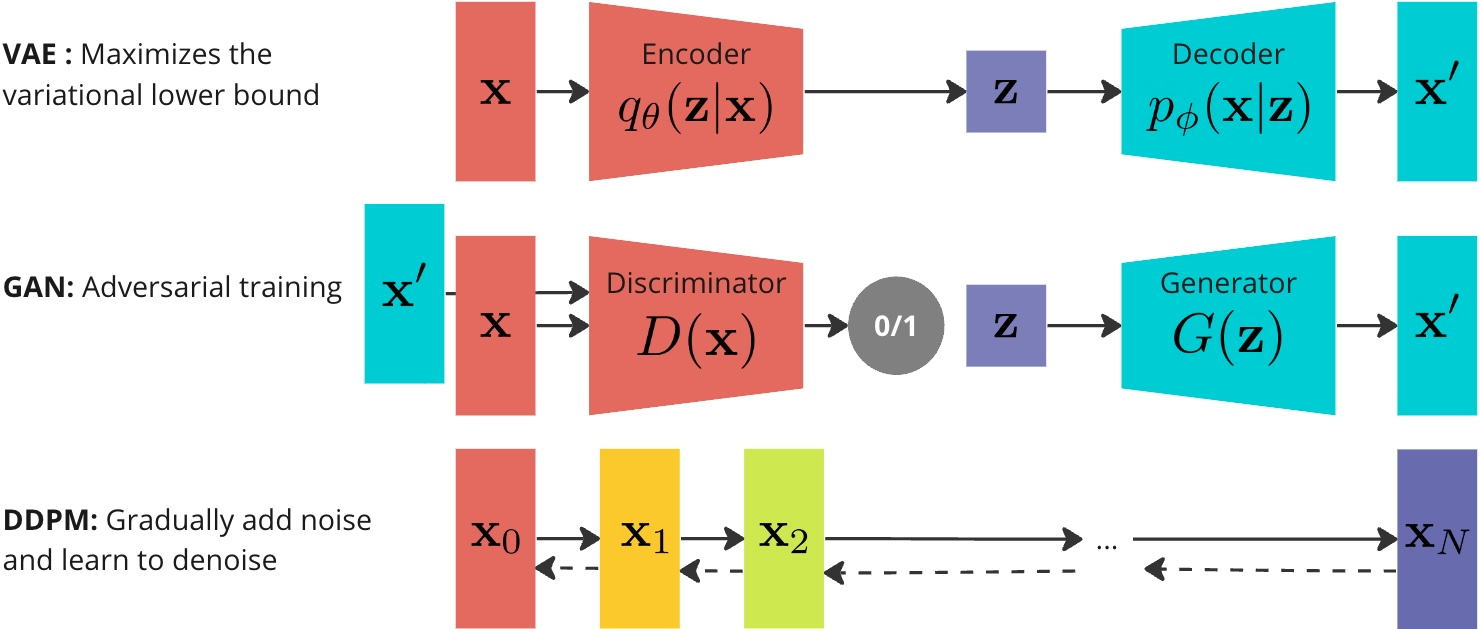
\includegraphics[width=1.0\linewidth]{images/related/generative_models_overview.jpg}
      \end{center}
      \caption{Overview of three families of generative models used in this work.}
      \label{fig:gen_models}
  \end{figure}


\subsection{Variational Auto-Encoders}

Introduced by  \cite{Kingma2014} and \cite{pmlr-v32-rezende14}, \ac{VAE}s are based on the variational 
inference framework. This framework will be presented here and then later be brought to the context of \ac{DL}.

\paragraph{VAE Framework}
Let's consider a dataset of observations $x \in \mathcal{D_X}$, a prior distribution of unobserved latent 
variables $p(z)$. The joint probability of this model can be written as $p(x,z) = p(x|z)p(z)$. The goal of 
\emph{variational inference} is to \emph{infer} good values of the latent variables and calculate the posterior
(intractable) $p(z|x)$. 

% Using Bayes theorem, we have:
% \begin{equation}
%       p(z|x) = \frac{p(z, x)}{p(x)}
% \end{equation}
% However, $p(x)$ is intractable, since we would need to compute it using all possible configurations of latent 
% variables. Thus, we need a way to approximate this posterior. 


Variational inference approximates the posterior with a family of distributions, typically multivariate 
Gaussian distributions, noted as $q_\lambda(z|x)$. To measure the similarity between the variational 
posterior $q_\lambda(z|x)$ and the true posterior $p(z|x)$, we can use the \ac{KL} divergence which measures
the similarity between two distributions. However, $\mathrm{KL}(q_\lambda(z|x) || p(z|x))$ is again intractable.

% We thus want to minimize:

% \begin{equation}
%       \mathbb{KL}(q_\lambda(z|x) || p(z|x)) = \mathbb{E}_q[\log q_\lambda(z|x) ] - \mathbb{E}_q[\log p(z|x) ] + \log p(x)
% \end{equation}

% However, this term is intractable because it again depends on $p(x)$.

The marginal log-likelihood can be decomposed as follows:

\begin{equation}
      \label{VAE_px_definition}
      \log p(x) = ELBO(\lambda) + \mathrm{KL}(q_\lambda(z|x) || p(z|x))
\end{equation}

with 

\begin{equation}
      ELBO(\lambda) = \mathbb{E}_{q_{\lambda(z|x)}}[\log p(x|z)] - \mathrm{KL}(q_\lambda(z|x) || p(z))
\end{equation}

Because the \ac{KL} divergence is always positive,  minimizing the right term in 
Eq.~\ref{VAE_px_definition} (which is intractable) is equivalent to maximizing $ELBO(\lambda)$, which is tractable. 
Indeed, $ELBO(\lambda)$ is a lower bound on the the marginal log-likelihood of the observed data $\log p(x)$.

\paragraph{DNN Context}
In the context of \ac{DL}, we parameterize the approximate posterior $q_\theta(z|x)$ with an encoder network which 
takes as input an image and outputs the parameters to a probability density. This 
is typically a multivariate Gaussian distribution, defined by a mean $\mu_\theta$ and standard deviation $\sigma_\theta$. Sampling from this 
distribution gives us a latent vector $z$. Similarly, we parameterize the likelihood $p_\phi(x|z)$ with a decoder 
(generative network), which takes as input a latent vector $z$ and outputs parameters of the data distribution.
For practical purposes, this distribution is typically a set of independent Bernouilli parameters or a multivariate 
Gaussian with fixed variance. In this way, the decoder
network simply outputs the reconstructed image directly.
The parameters $\theta$ and $\phi$ are the weights to the 
encoder and decoder respectively, and can be optimized via gradient descent. Note that when sampling a 
latent vector $z$ from the output given by the encoder, we perform a \emph{reparametrizaton trick} which 
allows us to backpropagate through the encoder network. This consists in sampling a random vector 
$\epsilon \sim \mathcal{N}(0, I_d)$ and then reparameterizing to obtain the latent vector $z$ with 
$z = \mu_\theta +  \sigma_\theta * \epsilon $. The basic architecture can be visualized in the 
first row of Figure \ref{fig:gen_models}.

% \begin{figure}[tb]
%       \begin{center}
%           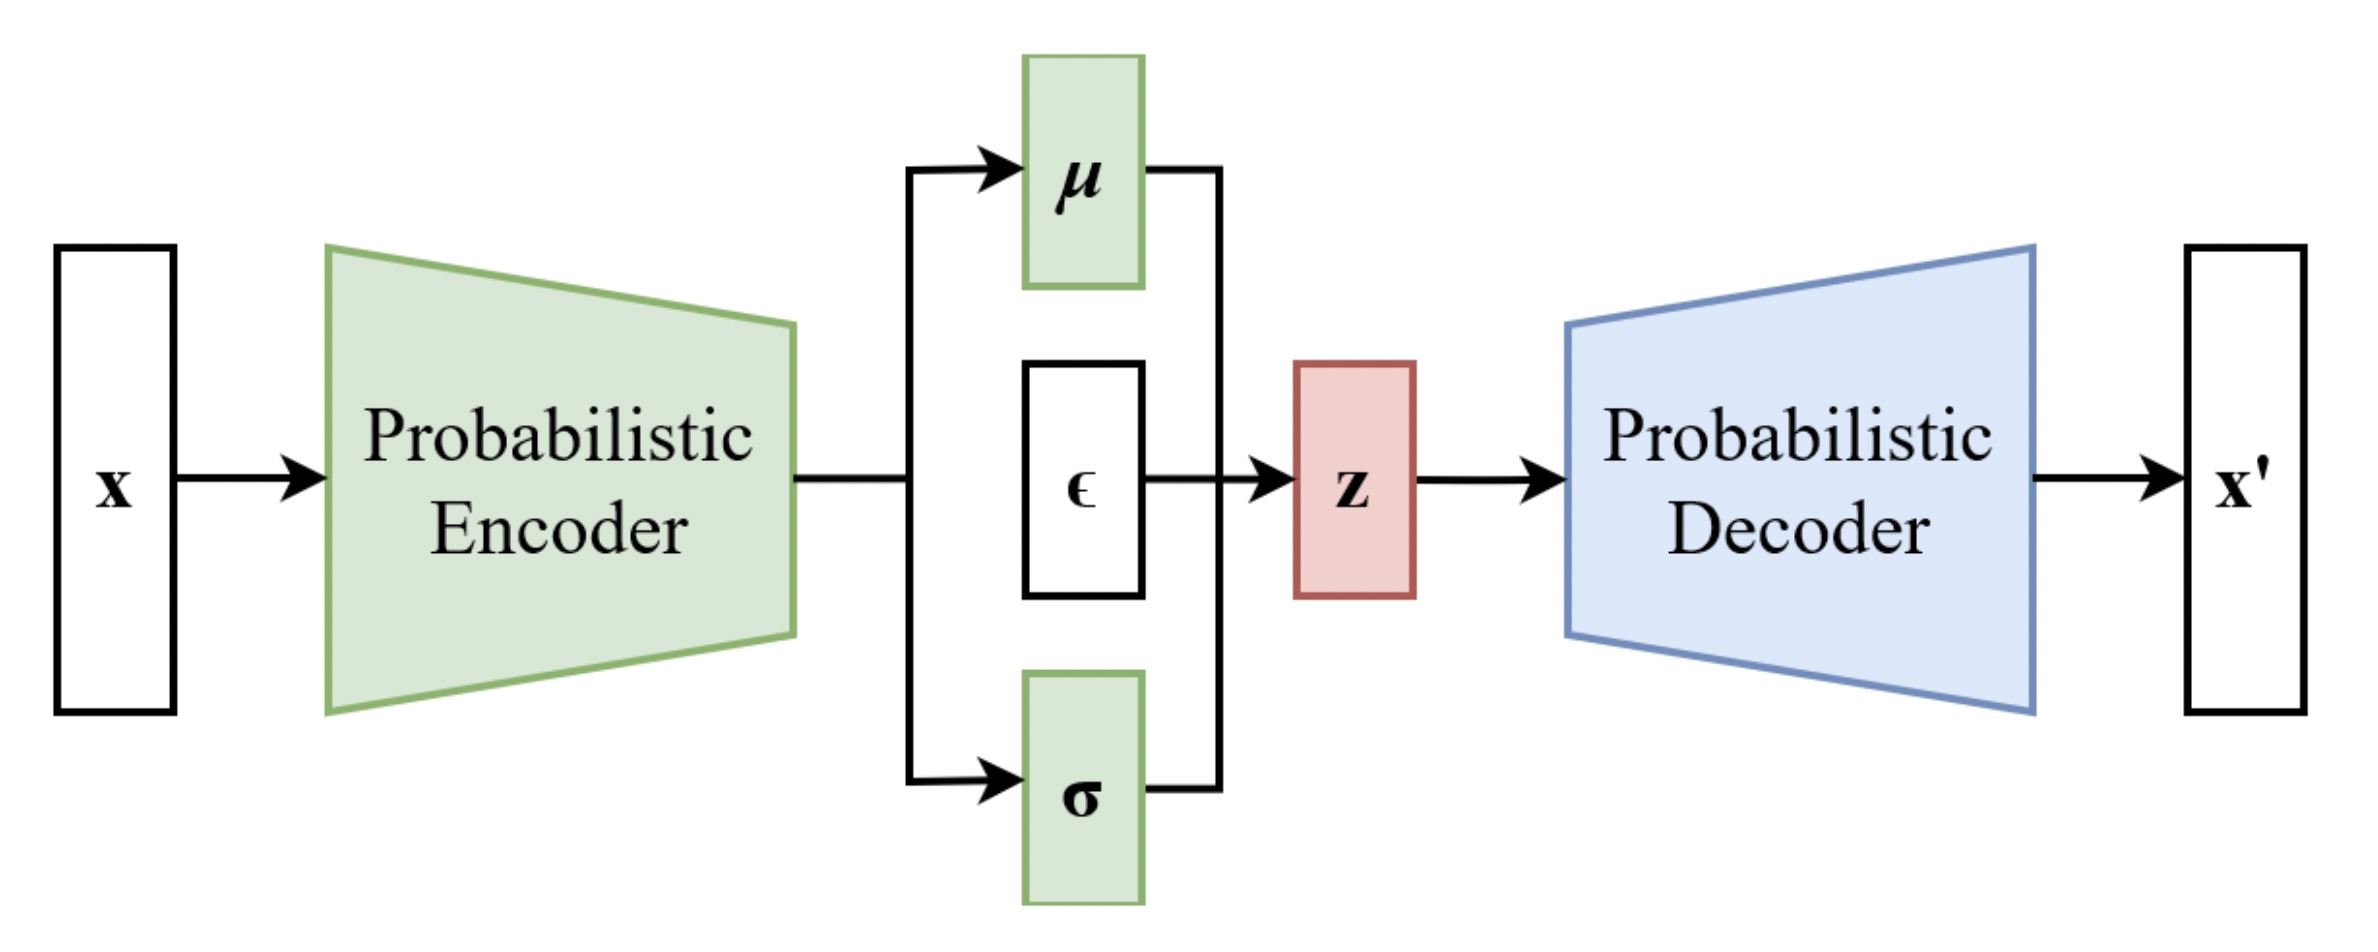
\includegraphics[width=1.0\linewidth]{images/related/vae.jpg}
%       \end{center}
%       \caption{Basic VAE architecture, using reparameterization trick.}
%       \label{fig:vae}
%   \end{figure}

We minimize the following loss function:

\begin{equation}
      L = \frac{1}{N}\sum_{i}^{N}l_i
\end{equation}

where 

\begin{equation}\label{eq:vae}
      l_i(\theta, \phi) = -ELBO(\theta, \phi) = - \mathbb{E}_{q_\theta(z|x_i)}[\log p_\phi(x_i | z)] + \mathrm{KL}(q_\theta(z|x_i)||p(z))
\end{equation}

and $N$ is the number of datapoints. 

The left term can be seen as the \emph{reconstruction loss}, which refers to how well 
the \ac{VAE} manages to reconstruct a given image. The right term can be seen as a 
regularizer which encourages the learned latent space to be meaningful. Without this 
regularizer, the encoder could assign a unique location for each image in the dataset. 
Although this would be easier to decode, the learned representation of the latent 
would not be \emph{meaningful}, which is one of our goals when learning this 
deep representative space.
 A meaningful latent space implies that two datapoints close 
in the latent space are also close in the image space. 


\paragraph{Disentanglement}\label{sec:disentanglement}

In fact, \cite{higgins2017betavae} show that when putting more penalty on the 
the \ac{KL}-divergence term in Equation \ref{eq:vae}, known as $\beta$-VAE, the \ac{VAE}
produces \emph{disentangled} representations. Disentanglement refers to a learned 
latent space in which each latent factor is mapped to an 
independent generative factor. For example, in a disentangled represenation, 
 one latent factor could control rotation 
while another one could control size. A disentangled latent space can be especially attractive 
in the case of image editing, which will be discussed later in \ref{subsection:latent_space_manipulation}.

\subsection{Generative Adversarial Networks}\label{sec:gans}

% \todo{talk about BigGAN and imagenet}

We will now introduce \ac{GAN}s, a framework introduced by \cite{goodfellow2014gan}
which has been become a core component in image generation and image editing applications. 


In contrast with \ac{VAE}s, \ac{GAN}s do not explicity model the probability 
distribution of the data $p(x)$. Instead, \ac{GAN} use two networks, the generator $G$ 
and the discriminator $D$ which are trained together adversarily. Similarly to 
\ac{VAE}, we use a latent space ${z \in \mathcal{Z}}$ which will be used as input for the 
generator network. Unlike \ac{VAE}s, this latent space is not learned, and is 
typically defined as $\mathcal{N}(0, I_d)$, with $d$ the dimension of the latent space. 

Concretely, the 
objective function of \ac{GAN}s is posed as a zero-sum game between $D$ and $G$, defined 
as follows:
\begin{equation}\label{eq:gan_objective}
      \min_{G}\max_{D}\mathbb{E}_{x\sim p(x)}[\log(D(x))] + \mathbb{E}_{z\sim p(z)}[\log(1 - D(G(z)))]
\end{equation}

For the discriminator, the goal is posed as a binary classification problem: 
correctly classify the real images from $p(x)$ as well as the fake images generated 
from $G(z)$. The generator has the opposite objective and "wants" to produce 
images that cannot be easily classified by the discriminator. 

Minimizing Equation \ref{eq:gan_objective} is equivalent to minimizing the \ac{JSD} between the 
distribution of real images and distribution of fake images. However, 
training GANs in practice is not straightforward, for reasons we will examine here.

\subsubsection{GAN Architecture}\label{sec:gan_architecture}
When referring to \ac{GAN}s, we typically refer 
to the training mechanism using the zero-sum \emph{GAN loss} (Equation \ref{eq:gan_objective}). This requires 
some generative network and a discriminator network trained jointly, but there is no further constraint on the 
architecture used by a \ac{GAN}.  Indeed, a \ac{VAE}'s decoder architecture can be practically identical
to a \ac{GAN}'s generator network, both transforming a latent vector $z$ into an image. Similarly, the 
discriminator can simply ressemble a CNN-classifier architecture. 
For this reason, there is nothing stopping us from having hybrid architectures which combines the 
typical encoder-decoder of a 
\ac{VAE} with a discriminator and a \ac{GAN} loss, as has been done by several works \citep{larsen2016autoencoding, 
xian2019f, esser2021taming}. In the case of images, Figure \ref{fig:dcgan} shows a typical \ac{GAN} architecture based 
on a \ac{CNN}, coined \ac{DCGAN} \citep{dcgan}. This basic architecture uses upsampling blocks 
(composed of deconvolutional layers) for the generator and downsampling blocks (composed of convolutional layers)
for the discriminator, which further works build off from. 

\begin{figure}[tb]
      \begin{center}
          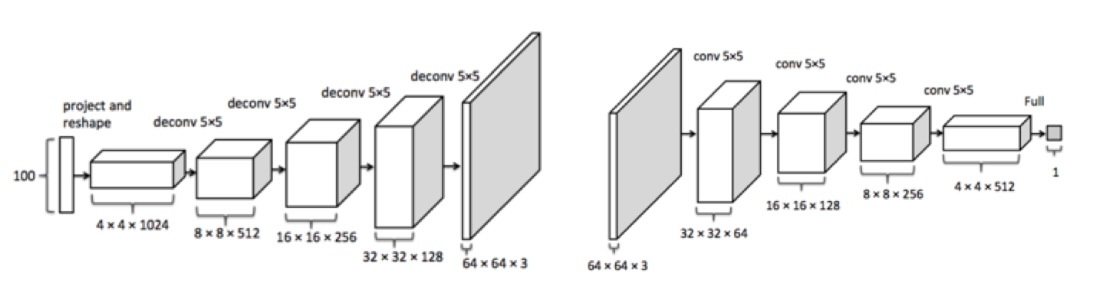
\includegraphics[width=1.0\linewidth]{images/related/dcgan.jpg}
      \end{center}
      \caption{DCGAN architecture. Generator (left) uses upsampling blocks with deconvolutional layers while the discriminator 
      (right) is a mirror image of the generator and uses downsampling blocks composed of convolutional layers.}
      \label{fig:dcgan}
  \end{figure}


\subsubsection{GAN Weaknesses}\label{subsubsection:gan_weaknesses}

\minipar{Training Instability}
In theory, we can expect to optimize Equation \ref{eq:gan_objective} by first optimizing $D$ 
optimally before optimizing $G$. In practice, however, training \ac{GAN}s is effectuated 
by alternating gradient descent steps to the discriminator and generator. 
However, GANs are prone to important training 
instability. 

One of the most notable issues when optimizing Equation \ref{eq:gan_objective} by alternating 
gradient descent steps is training collapse due to a too-strong discriminator. \cite{arjovsky2017towards}
shows that in the case of image generation, a "perfect" discriminator exists which can perfectly 
separate real data from fake data. What's worse, as the discriminator gets stronger, 
 the gradients  given to the generator will vanish \citep{arjovsky2017towards}. 
 This means, of course, that training collapses, since the generator can no longer improve. 
 It's important to note that this gets exacerbated in the case of high-resolution synthesis. 
 Indeed, while high-resolution images improves discriminability \citep{pmlr-v70-odena17a}, high-resolution 
 synthesis becomes a harder task for the generator \citep{karras2018progressive}. Moreover, in the case of 
 high-resolution synthesis, the size of the mini-batch must be smaller (since the images are more memory-intensive)
 and thus the generator has even guidance from the gradients. The \ac{GAN}'s training stability 
and the \ac{GAN}'s capacity to generate high-resolution images thus goes hand-in-hand. Although the 
reverse problem could also occur in practice (a strong generator which too-easily tricks the discriminator, causing 
the discriminator "stuck" during learning), 
this occurs less often given the fact that the discriminator's job is inherently easier.

\minipar{Mode Collapse} Mode collapse refers to the generator collapsing to only produce one sample or one family of
similar samples. In this case, a single genered sample which is classified as realistic by the discriminator will 
push the generator towards this sample. Indeed, the samples are treated independently, and the generator will have no penalty 
in producing similar samples. 

\minipar{Unstructured latent space}
Because the latent space is fixed instead of learned, the latent space of a GAN can be unstructured 
and typically entangled. Although not problematic in itself, it can be prohibit or limit 
fine-grained control for generation or manipulation.

\minipar{No inference for z} Because a \ac{GAN} typically lacks an encoder network (with the exception of hybrid \ac{VAE}s/\ac{GAN}s
as mentioned in \ref{sec:gan_architecture}), we cannot easily obtain the latent \ac{GAN} code 
corresponding to a real image. This makes high-level image editing problematic. 

The works and techniques descibed below ultimately allowed \ac{GAN}s to become state-of-the-art in image synthesis.


\subsubsection{GAN Improvements}

We will now discuss some recent advances which address the aforementioned weaknesses as well as the 
recent works which finally allowed very high-resolution synthesis.

\minipar{Non-saturating GAN loss} The non-saturating GAN loss, introduced in the original \ac{GAN}
paper \citep{goodfellowgans} changes the objective of the 
generator from Equation \ref{eq:gan_objective} to:

\begin{equation}\label{eq:non_saturating}
      \min_G \mathbb{E}_{z \sim p(z)}[-\log(D(G(z)))]
\end{equation}

This reframes the initial goal posed by Equation \ref{eq:gan_objective}. Instead of minimizing the 
probability that the generated samples are 
classified as fake, Equation \ref{eq:non_saturating} maximizes the probability that the generated 
samples are real. This objective provides stronger gradient information to the generator early in 
training and aims to treat the vanishing gradients problem evoked above. Although this change in 
objective does indeed help for vanishing gradients, gradients still become very noisy with little
value to the generator when the discriminator becomes too strong \citep{arjovsky2017towards}.


\minipar{Minibatch Discrimination}
Minibatch discrimination, introduced by \cite{improved_techniques_gans}, consists in providing 
extra information to the discriminator regarding the variety of the samples in the current mini-batch. 
Concretely, for a single sample, we calculate its distance (in a feature space) to all the other samples, 
 sum these distances and concatenate this value to the generated sample $x_i$. Other work uses a variant of 
 this by performing standard deviation in the feature space and concatenates these values to the input of 
 the discriminator \citep{karras2018progressive}. Because the discriminator will 
 have access to extra information (very small distances correlate with fake samples), the generator will 
 be encouraged to produce diverse samples. 

 \minipar{Spectral Normalization} Introduced in \cite{miyato2018spectral}, spectral normalization 
 consists in constraining the weights of the discriminator during training. This improves 
 gradient flow during training and helps stability of training.

\minipar{Progressive Growing of GANs}\label{par:progressive_growing}
In 2017, Karras introduced \ac{PGGAN} \citep{karras2018progressive}, which further tackles GANs' instability problems 
specifically for the goal of high-resolution image resolution. This was the first GAN architecture which successfully 
managed to generate high-quality images of $1024 \times 1024$ resolution. The intuition is straightforward: instead 
of brutally generating high-resolution images which is prone to heavy instability for the reasons mentioned above,
 the generator and discriminator should be trained 
\emph{progressively} from low-resolution generation to high-resolution generation. Figure \ref{fig:pgan}
shows the training mechanism for this architecture.
 The generator and discriminator, mirror architecures of 
each other, are first trained to successfully generate $4 \times 4$ resolution images. This is an easy 
task for the generator, and is successfully trained without much training difficulty. When training is 
complete, another upsampling and downsampling block are respectfully added to the 
generator and discriminator. 
At each new addition of a new block, the generation gradually blends a simple nearest-neighbor 
upsampling of the previous layer with the generation of the newly trained network. As training converges (visually or 
by some pre-defined metric), a new block of layers are added to the discriminator and generator. Because at each new 
addition of an upsampling block, the generator's weights are already at decent starting points, 
the gradients from the discriminator are more likely to be able to guide the generator in the right direction.

Later work \citep{karnewar2020msg, karra2020stylegan2} builds off this framework in a single 
architecture which implicitly performs progressive-growing without explicitly changing the architecture at each new 
resolution adition. 

\begin{figure}[tb]
      \begin{center}
          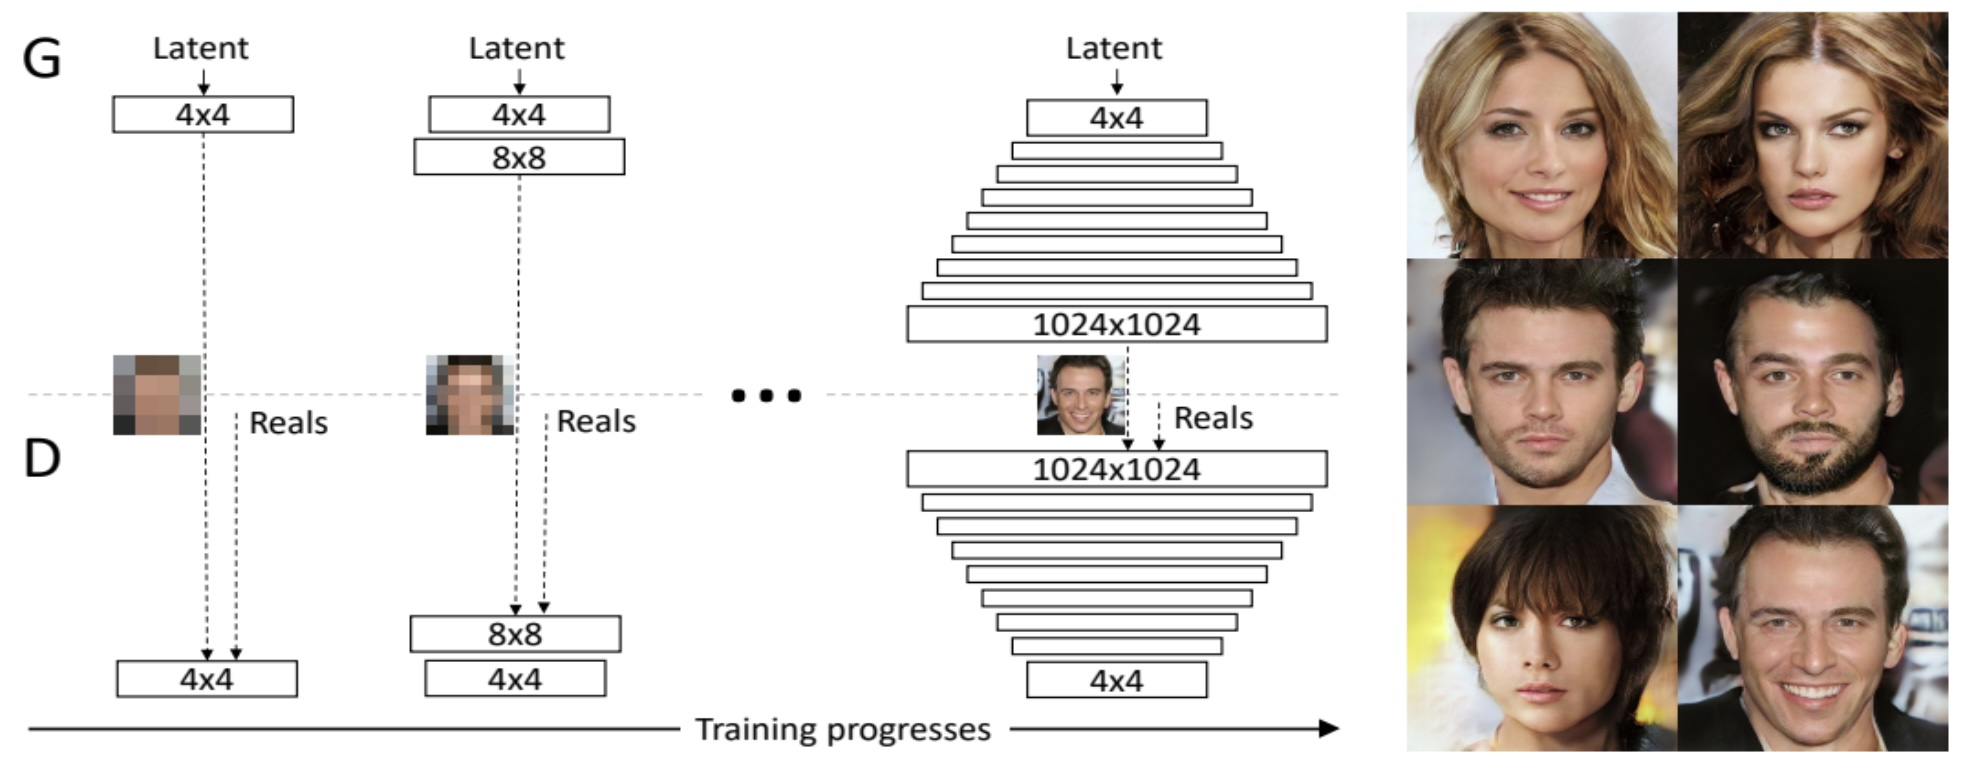
\includegraphics[width=0.7\linewidth]{images/magec/pgan.jpg}
      \end{center}
      \caption{Progressive Growing of GANs. Figure taken from \cite{karras2018progressive}}
      \label{fig:pgan}
  \end{figure}
  

\minipar{A learned and disentangled latent-space}\label{par:latent_space}
Introduced in 2020, StyleGAN \citep{karra2019stylegan} and later StyleGAN2 \citep{karra2020stylegan2}
revolutionized \ac{GAN} synthesis by introducing a new latent space which is learned, rather than the 
typical fixed $\mathcal{N}(0,1)$. Figure \ref{fig:stylegan} summarizes this architecture. We define a 
simple \ac{MLP} network which maps the mapping latent vector from the $\mathcal{N}(0,1)$ space to a new 
learned $\mathcal{W}$ space. This latent code is first projected to another space (the $A$ blocks 
in Figure \ref{fig:stylegan}) and
 then modulates the feature maps via \ac{AdaIN} layers \citep{huang2017arbitrary}, given by the following 
 equation:

 \begin{equation}
      \text{AdaIN}(\mathbf{x}_i, \mathbf{y}) = \mathbf{y}_{s, i}\frac{\mathbf{x}_i - \mu(\mathbf{x}_i)}{\sigma(\mathbf{x}_i)} + \mathbf{y}_{b,i}
 \end{equation}

where $\mathbf{x_i}$ is the $i^{\text{th}}$ feature map in the current layer and $\mathbf{y}$ is 
the learned style parameters for the current block. 

Because each feature map is normalized via the \ac{AdaIN} operation, only the current style at the 
current scale-specific block controls the modification at this level. To further encourage 
styles to localize, \cite{karra2019stylegan} performs \emph{mixing regularization} during training, 
where two different latent codes $\mathbf{w}_1$ and $\mathbf{w}_2$ are mixed at some crossover point 
when synthesizing an image. Moreover, the learned latent 
space naturally encourages disentanglement of high-level image features. This localized latent space
allows a truly controllable image synthesis. Observe 
Figure \ref{fig:stylegan_styles} for example, which shows that by mixing two different style codes 
$\textbf{w}_1$ and $\textbf{w}_2$ (which respectfully generate image $A$ and $B$
through StyleGAN) 
at some cross-over point, we can transform $A$ using coarse, 
medium, or fine-grained styles from $B$. 

In later work, \cite{karra2020stylegan2} improves upon this work by improving the 
architecture, improving the modulation and demodulation scheme of \ac{AdaIN} and adding 
\emph{perceptual path regularization} for even more smoothness in the latent space. 
This encourages for small changes in the latent space to produce small changes in the 
image space. With these improvements, StyleGAN2 quickly became the state-of-the-art 
in image generation for constrained datasets like faces \citep{celeba,karras2018progressive},
 bedrooms and animals \citep{lsun} for many years to come. Moreoever, with its 
 powerful latent space, StyleGAN2 opened the door for many works on image editing, 
 more of which will be discussed in \ref{section:image_editing}.
 

\begin{figure}[tb]
      \begin{center}
          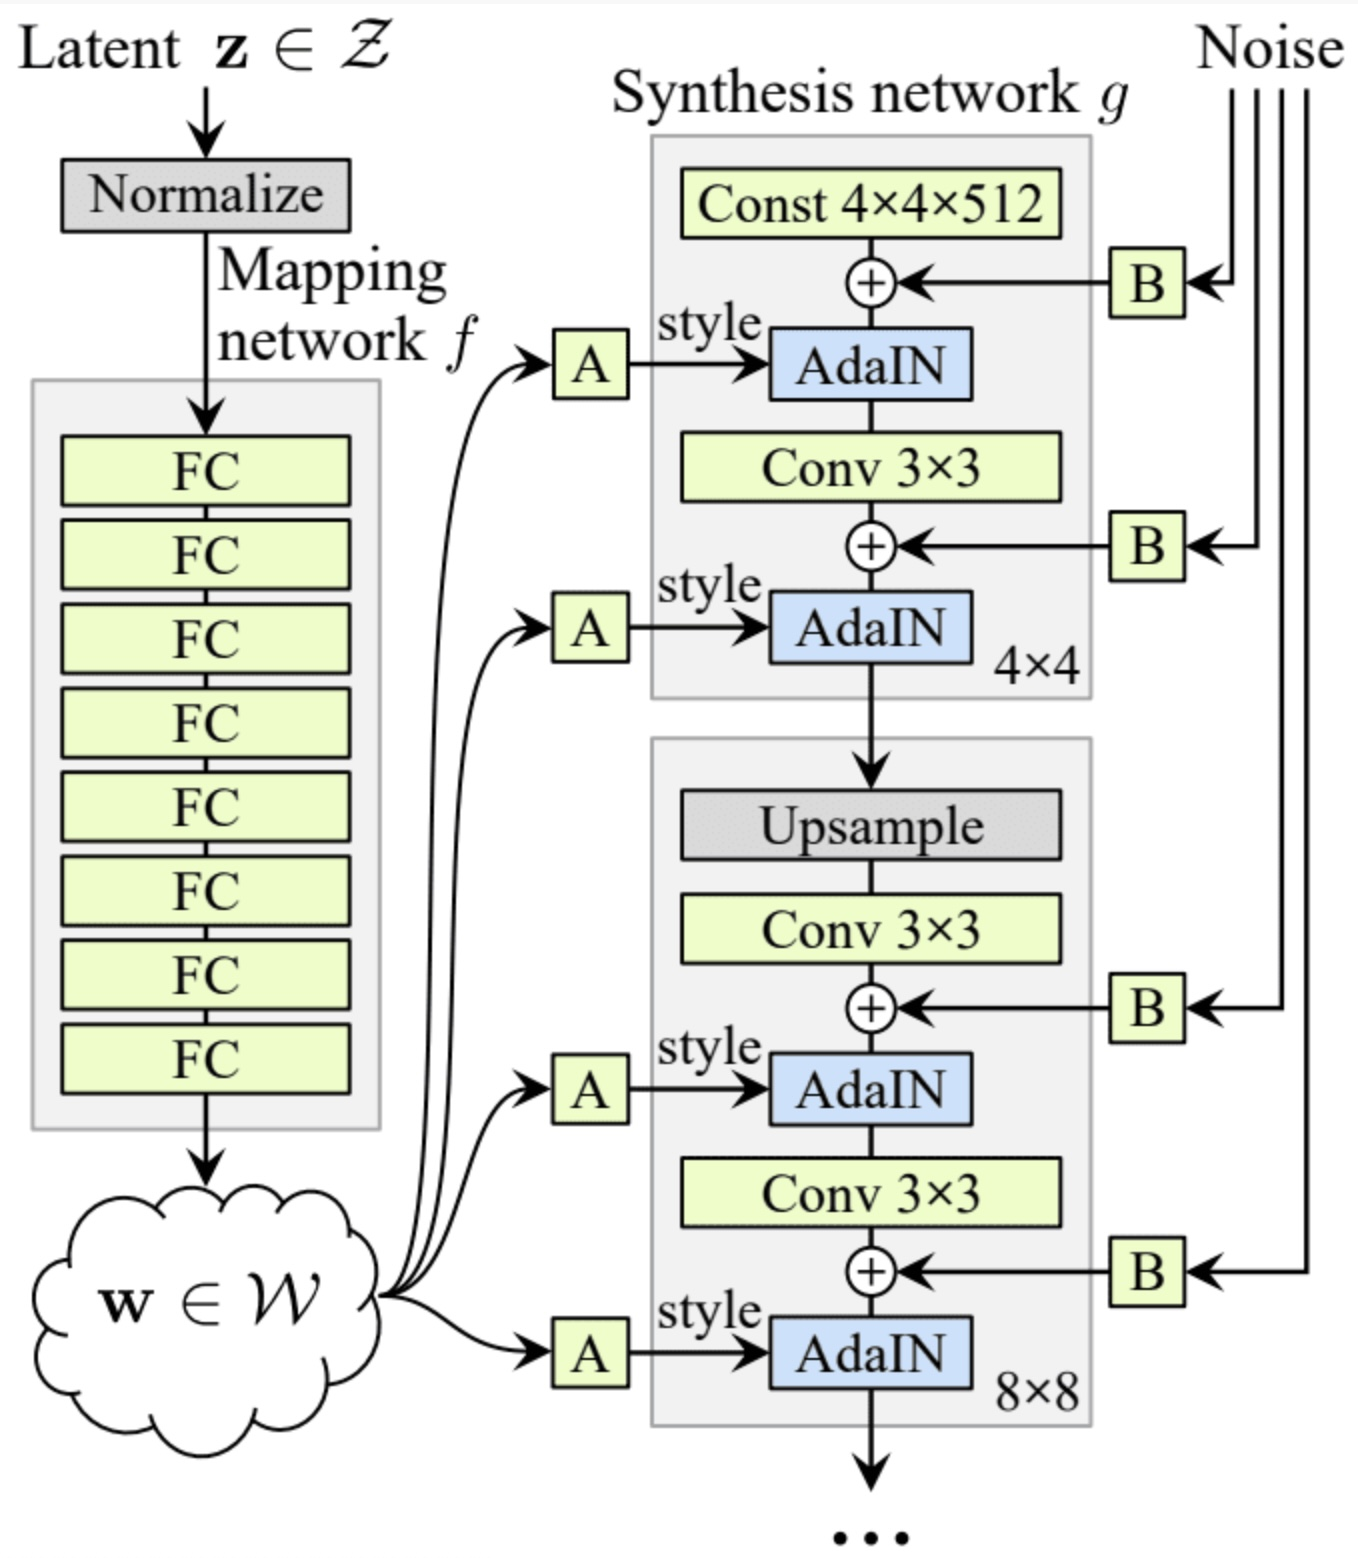
\includegraphics[width=0.5\linewidth]{images/related/stylegan.jpg}
      \end{center}
      \caption{StyleGAN architecture. Figure taken from \cite{karra2019stylegan}.}
      \label{fig:stylegan}
  \end{figure}

  \begin{figure}[tb]
      \begin{center}
          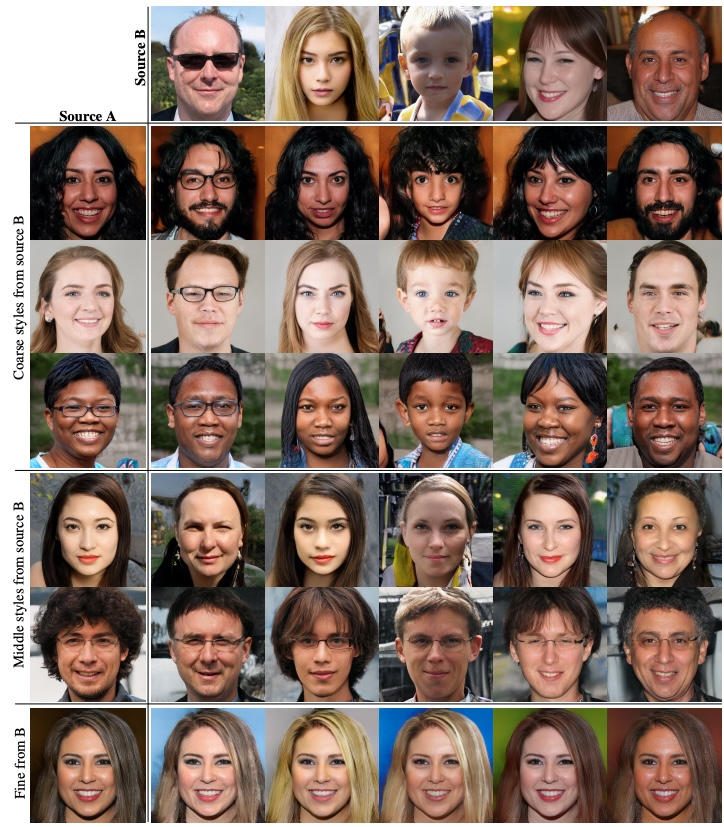
\includegraphics[width=0.7\linewidth]{images/related/stylegan_styles.jpg}
      \end{center}
      \caption{Synthesis control from latent space manipulation. Figure taken from \cite{karra2019stylegan}}
      \label{fig:stylegan_styles}
  \end{figure}

\subsubsection{Conditional GANs}
\ac{GAN}s can be conditioned on some condition $c$, known as \ac{cGAN}s \citep{mirza2014conditional}.
\ac{cGAN}s condition both the generator and discriminator on the condition, and Equation \ref{eq:gan_objective}
can be rewritten as follows:

\begin{equation}\label{eq:gan_objective}
      \min_{G}\max_{D}\mathbb{E}_{x, c\sim p(x, c)}[\log(D(x, c))] + \mathbb{E}_{z\sim p(z), c\sim p(c)}[\log(1 - D(G(z, c), c))]
\end{equation}

The condition can be a class label, a vector, or an image. The latter case is known as image-to-image translation,
and will be discussed in more detail in section \ref{subsection:image-to-image models}.
Although unconditional \ac{GAN}s achieved remarkable, photo-realistic synthesis on restricted datasets
like faces, conditional  \ac{GAN}s historically struggled on more diverse datasets like ImageNet. 
In 2019, however, significant progress on this front was made with BigGan \citep{brock2018large}, 
which achieved state-the-art results on ImageNet, significantly outperforming previous methods. They 
used a residual architecture, \ac{GAN} hinge loss \citep{lim2017geometric} (a variant of the adversarial loss),
 spectral normalization \citep{miyato2018spectral},
and class-conditional Batch Normalization \cite{ioffe2015batch}, scaling up the layer sizes, 
and increasing 
batch size significantly improves performance. BigGAN remained state-of-the-art for
 ImageNet synthesis 
for several years until diffusion models outperformed them, which we describe in the
 next section. 



\subsection{Denoising Diffusion Probabilistic Models}\label{sec:diffusion:models}

Although \ac{DDPM}s have roots dating from earlier years \citep{sohl2015deep}, the model became 
especially prominent in 2020 by \cite{ho2020denoising}, using a UNet architecture 
as the denoiser, which has since become standard practice. \cite{ho2020denoising} acheived 
similar results to their 
\ac{GAN} counterparts for various datasets. Then, \cite{dhariwal2021diffusion} adapted 
the model and achieved state of the art results on ImageNet and various LSUN datasets like 
Bedrooms, Horses and Cats, outperforming BigGAN \citep{brock2018large} and StyleGAN \citep{karra2020stylegan2}. 
Recently, \ac{DDPM}s achieved image synthesis from free-form text of remarkable quality \citep{ramesh2022hierarchical, nichol2021glide, saharia2022photorealistic, gafni2022make, rombach2022high}, 
These models capture complex intrinsic knowledge about the world from the billions of images used to train them \citep{schuhmann2022laion}, which 
allows high-quality generation of even completely imaginary concepts, like "a dragon fruit wearing karate belt in the snow."

In this section, we will first present the general framework of diffusion models. Then, we will 
present their conditional variant and techniques used to improve synthesis quality. Finally, 
we will go into more detail of some of the recent prominent models which have achieved photo-realistic 
results.

\subsection{Framework}

Introduced by \cite{sohl2015deep} and imporved by \cite{ho2020denoising}, the \ac{DDPM} is a class 
of generative models trained to remove various levels of noise added to an input training image, as illustrated in Fig.\ref{fig:gen_models}.
Given an input image $\x_0$, the \emph{forward process} refers to the creation of the latent variables 
$\x_1, ..., \x_T$ by gradually noising the latents incrementally with gaussian noise, controlled by 
a variance schedule ${\beta_t}$ which grows from $0$ to $1$. Note that the schedule of 
$\beta_t$ is an implementation choice: \cite{ho2020denoising} proposed a linear schedule while 
\cite{dhariwal2021diffusion} proposed a cosine-based schedule which improved performance.

Concretely:

\begin{equation}
      \x_t = \sqrt{1 - \beta_t} \x_{t-1} +  \sqrt{\beta_t} \epsilon
\end{equation}

By posing $\alpha_t = \prod_{i=1}^{T} (1 - \beta_i)$ and through reparameterization, 
a nice property of \ac{DDPM}s is that we can always express a latent map $\x_t$ in relation 
to the initial image $\x_0$:

\begin{equation}
      \x_t = \sqrt{\alpha_t} \x_0 +  \sqrt{1 - \alpha_t} \epsilon
\end{equation}

Where $t$ varies from $0$ to $T$ and determines the mixing coefficient $\alpha_t$, which monotonically 
decreases from  $\alpha_0 = 1$ (no noise) to $\alpha_T \simeq 0$ (almost pure noise) for a large integer $T$.


The \emph{reverse process} refers to learning a model  $\epsilon_\theta$  which approximates the noise added at a given 
timestep $t$. Specifically, \ac{DDPM}s are trained with the following objective:

\begin{equation}
      \mathcal{L} = \displaystyle \mathbb{E}_{\x_0, t, \epsilon} \Vert \epsilon - \epsilon_\theta(\x_t, t) \Vert_2^2,
\end{equation}


% This training is performed for different values of the mixing coefficient $\alpha_t$, monotonically decreasing from $\alpha_0 = 1$ (no noise) to $\alpha_T \simeq 0$ (almost pure noise) for a large integer $T$.



% The level 
% of noise is determined by a timestep $t$, which varies from $0$ (no noise) to a large integer $T$ (pure gaussian noise).

% % Given a datapoint sampled from a real data distribution $\mathbf{x}_0 \sim \mathcal{D}_\mathcal{X}$, 


% \ac{DDPM}s \citep{ho2020denoising} is a class of generative models trained with the following image denoising objective:

% \begin{equation}
%     \mathcal{L} = \displaystyle \mathbb{E}_{\x_0, t, \epsilon} \Vert \epsilon - \epsilon_\theta(\x_t, t) \Vert_2^2,
% \end{equation}
% where $\epsilon_\theta$ is a noise estimator network trained to predict the noise $\epsilon \sim \gaussian$  an input image $\x_0$ in the following way: $\x_t = \sqrt{\alpha_t} \x_0 +  \sqrt{1 - \alpha_t} \epsilon$. This training is performed for different values of the mixing coefficient $\alpha_t$, monotonically decreasing from $\alpha_0 = 1$ (no noise) to $\alpha_T \simeq 0$ (almost pure noise) for a large integer $T$.

\minipar{Sampling}

At inference time, a new sample from the training distribution can be obtained by starting from 
random Gaussian noise $\mathbf{x}_T \sim \mathcal{N}(\mathbf{0}, \mathbf{I})$, and iteratively
refining it with the noise estimator network with the following equations, called 
\textit{DDPM sampling equations} \citep{ho2020denoising}:

\begin{align*}
      \hat{\x}_0 &= \frac{1}{\sqrt{\alpha_t}}(\x_t - \sqrt{1 - \alpha_t} \cdot \epsilon_\theta(\x_t, t)) \\
      \x_{t-1} &= \frac{(\alpha_{t-1}-\alpha_t) \sqrt{\alpha_{t-1}}}{\alpha_{t-1}(1 - \alpha_t)} \hat{\x}_0 + \frac{(1-\alpha_{t-1})\sqrt{\alpha_t}}{(1 - \alpha_t)\sqrt{\alpha_{t-1}}} \x_t + \sigma_t \z
\end{align*}

where $t$ goes from $T$ to $1$, 
$\sigma_t$ is a variance parameter (either learned or fixed), and $\z \sim \gaussian$.
In practice, the noise estimator network is modelled as a UNet \citep{ronneberger2015UNet} 
which inputs the noise map $\x_t$ concatenated with the timestep embedding of $t$. 


Without any modification, sampling with diffusion models is very costly, as it requires $T$
(which is usually on the magnitude of several thousands) forward passes to generate an image, a much slower 
process than their \ac{GAN} counterparts which only require one forward pass. On a modern 
GPU, a single sampling takes several minutes. \cite{nichol2021improved} shows that we can 
resample the number of steps and obtain their corresponding variances and perform fewer 
sampling steps during inference. They show that $100$  steps is sufficiant for high-quality 
generation with their model trained with $4000$ steps. \cite{song2021denoising} show that 
this strategy works even better with a deterministic model, and can reduce the amount of steps
down to $~20$. Finally, \cite{rombach2022high} show that we can considerably reduce training and 
inference complexity by working with latents $\x_t$ in a compressed space rather than 
the original image dimensions.

\subsection{Conditional DDPMs}\label{subsection:conditional_ddpm}

Conditional diffusion models \citep{chen2021wavegrad, saharia2022image, saharia2022palette}
make the denoising process conditional on a signal. Like other conditional generative models, 
this can be  a text, image, segmentation map, etc. In practice, the conditioning is 
typically done with concatenation to the noise map for modalities other than text, 
while text typically conditions the generation in multiple layers of the 
UNet through attention mechanisms \citep{nichol2021glide, rombach2022high, saharia2022photorealistic}.

\paragraph{Classifier-Guidance}
% dhariwal2021diffusion ADM
To improve generation quality, \cite{sohl2015deep, song2020score, dhariwal2021diffusion} show that 
it's possible to make use of an auxiliary classifier
during sampling to further guide the generation towards the desired output. 
In particular, an auxiliary classifier $p_\psi(y|\x_t, t)$ can be trained on images of varying noise 
$(\x_t, t)$ 
and be then used to guide the sampling during inference with its gradient 
 $\nabla_{\x_t} \log(y|\x_t, t) $ further towards the class $y$. 
 \cite{nichol2021glide} similarly shows improved results by using the CLIP \citep{radford2021learning}
 model as the classifier.
% ADM; look

\paragraph{Classifier-free Guidance}
% ho2022classifierfree
\cite{ho2022classifierfree} improves upon classifier guidance by 
proposing classifier-free guidance. Instead of using an auxiliary classifier, 
classifier-free guidance uses the \ac{DDPM} itself to further guide the 
generation. Concretely, it consists in tweaking the training of a conditional \ac{DDPM} 
by dropping the text or class label for a percentage of the time (usually, $20\%$)
and instead train with a null-text token or null-class label $\emptyset$. Then, during 
sampling, the output of $\epsilon_\theta$ is extrapolated further in the direction 
of the class or text with:

\begin{equation}
      \hat{\epsilon_\theta}(\x_t|y) = \epsilon_\theta(x_t, \emptyset) + s \cdot (\epsilon_\theta(x_t, y) - \epsilon(x_t, \emptyset))
\end{equation}

\noindent where $s > 1$

\cite{nichol2021glide} shows the superiority of this guidance compared to classifier-guidance,
and classifier-free guidance is currently standard practice for conditional diffusion models.

\subsection{Prominent Diffusion Models}

Initially, unconditional or class-conditional diffusion models were trained on small 
datasets which allowed benchmarking against \ac{GAN}s \cite{ho2020denoising, dhariwal2021diffusion}.
Recently, works started to train diffusion models on very large billion-element text-image 
datasets \citep{schuhmann2022laion} which allowed unprecedented generation  in terms of 
photorealism and diversity. GLIDE \citep{nichol2021glide} built off the architecture in 
\cite{dhariwal2021diffusion} to adapt class-conditioning to text-conditioning. DALL-E 2 \citep{ramesh2022hierarchical}
also built on this architecture, but conditioned the generation on  CLIP \cite{radford2021learning}
encodings of the image to "unCLIP" the embedding. Imagen \citep{saharia2022photorealistic} a leveraged 
a much larger language model for the text encoder which conditioned generation, showing that 
performance scales with the text encoder size but not with the UNet size. Latent Diffusion Models \citep{rombach2022high}
first compresses images into a $~8\times$ reduced space with an encoder before performing the 
diffusion process on these latents, rather than the noised images. Their model requires much 
less ressources for training and also allows for a much faster inference speed. Other models, 
like MidJourney


\section{Image Editing}\label{section:image_editing}

Image editing is a particular case of image synthesis which requires (1) a way to use the 
input image as input and (2) a specific editing task. There are two ways to approach this 
problem: training/fine-tuning a network for the task (\ref{subsection:image-to-image models}) or 
leveraging a pre-trained network, which has already learned powerful semantics, and tweaking the 
internal feature-maps or latent code (\ref{subsection:hacking_generative_model}, \ref{subsection:latent_space_manipulation}).
We can look at these approaches from a "coarse-to-fine" point of view - image-to-image models (\ref{subsection:image-to-image models})
typically train an entire network from scratch to perform the task at hand, "hacking" generative models (\ref{subsection:hacking_generative_model})
manipulate a subset of internal feature-maps or weights from a pre-trained network, and latent space manipulation (\ref{subsection:latent_space_manipulation})
leave the entire network as is, only manipulating the latent code input. The approaches typically 
vary on the "controllability - practicality" tradeoff. That is, the less we manipulate a pre-trained 
network, the more tied we are to the original dataset the network was trained on. However, re-training 
a new network as is typical in image-to-image models requires much more data (which we may not have)
and training resources. For the "average" person, it is infeasible to train a model as semantically powerful as 
state-of-the-art generative models (Stable Diffusion \citep{rombach2022high}, for example, cost $\$160,000$ and 
$80,000$ A100 \citep{gpua100} hours to train \citep{MosaicML}). Moreover, state-of-the-art generative models 
intrinsically learn powerful concepts, which can be leveraged (see \ref{subsection:latent_space_manipulation}). 
To summarize, all the following approaches have their merits, and as a general "guideline", the more the 
input image deviates from the domain of a pre-trained model, the more tweaking (or new training) a user 
should do.

\subsection{Image-to-Image Models}\label{subsection:image-to-image models}
Image-to-image models can be seen as a straightforward way to perform image editing when 
we wish to "translate" an image from a source domain $A$ to a target domain $B$. In this case, the entire image is typically 
edited to (1) keep prominent structures of the source image and (2) belong to the target 
domain. Typical application of these include sketches to photos, photos to paintings, 
semantic maps to photos, colorization, etc. The task of inpainting, which consists in generating a missing 
part of an input image, is a particular case of image-to-image models and will be discussed in depth in 
Chapter \ref{chapter:gradpaint}. Image-to-image translation has almost exclusively been worked on using \ac{GAN}s except 
in recent works which 
adapted \ac{DDPM}s for the task. In the case where we have access to paired data  containing 
before and after images, \cite{pix2pix} proposed a general framework "Pix2Pix" using a \ac{cGAN} 
where both the generater and discriminator are conditioned by the input image as well as a fully-convolutional 
discriminator "PatchGAN", which discriminates patches as real or fake and then aggregates the results.
The authors 
proposed a UNet architecture with skip connections since the input and output images generally share 
many similar edges and features. The work used an $L1$ loss as well as a \ac{GAN} loss,  
encapsulating the two objectives stated above. Pix2PixHD \citep{wang2018pix2pixHD}
extended this framework for 
high-resolution images ($2048 \times 1024$). Pix2PixHD used a similar idea to Progressive Growing (see 
section \ref{par:progressive_growing}) and first trains a low-resolution generator before  
adding a high-resolution generator to the architecture, with both architectures remaining fully-trainable.
Multi-scale discriminators were also added for further training stability.
Later  \ac{GAN}-based works extended this, first with spatially-adaptive normalization layers \citep{gaugan} and then
later with a more powerful, spatially-aware discriminator which eliminates the need for a reconstruction loss \citep{sushko2020you}.
 More recently, \cite{psp} adapted the image-to-image framework by training 
an encoder-decoder network in which the encoder predicts latent codes of StyleGAN2 \citep{karra2020stylegan2}
to reconstruct the image. With restricted domains where StyleGAN2 excels, such as faces, this produces  
very natural results, unlike the Pix2Pix (and successors) frameworks, which are prone to artifacts.
Recently, conditional \ac{DDPM}s aborded the image-to-image translation tasks, such as super-resolution \citep{saharia2022image} and 
inpainting \citep{nichol2021glide}. \cite{saharia2022palette} provide a general image-to-image framework with \ac{DDPM}s, 
which builds upon the architecture from \cite{dhariwal2021diffusion} and concatenating the source image with 
the noise map at every denoising step, as described in \ref{subsection:conditional_ddpm}. 

In the case where we don't have access to paired data, different approaches exist. 
A straightforward approach consists in solely performing style transfer \citep{huang2017arbitrary}
for adapted cases, like photos to paintings. They use a fixed pre-trained VGG encoder \citep{simonyan2014very}
and a trainable decoder network which is trained with a content loss and a style loss (calculated by using 
the same VGG network). \cite{cyclegan} produced a novel approach, CycleGAN, which consists in training two \ac{GAN}s, 
along with a cyclic loss the translated source image translated back to the source domain should produce the 
initial source image.  \cite{choi2018stargan} and later \cite{choi2020stargan}
proposed a general framework for unsupervised image-to-image translation in the case of multiple domains. The works 
noted that generalizing a CycleGAN approach  would result in a quadratic amount of \ac{GAN}s to train.
Instead, \cite{choi2020stargan} trains one \ac{GAN}, in which the discriminator predicts scores for each domain, 
one style encoder, which outputs a style given an image, and one mapping function, which outputs a style given 
a source domain and a latent vector. The work conditions the generator with the style encoding
and allows realistic translations for multiple domains. Recent works with \ac{DDPM}s leveraged large and powerful 
pre-trained models for down-stream image-to-image translation tasks, requiring as little as 1000 labelled 
training data to perform high-quality image-to-image translation \citep{zhang2023adding, wang2022pretraining, voynov2022sketch}.

\subsection{"Hacking" a generative model}\label{subsection:hacking_generative_model}
We refer to "hacking" a generative model as manipulating the network's internal trained weights 
or feature maps in order to have fine-grained control of the output generation. These methods 
have roots in understanding how the internal structure of \ac{DNN}s affect their prediction \citep{collins2018deep, zeiler2014visualizing, strobelt2017lstmvis, karpathy2015visualizing, chen2019delving}.
\cite{bau2018gan} extended this to \ac{GAN}s, and showed that specific feature maps in a pretrained \ac{GAN}
corresponded to different concepts. After finding the specific feature maps, they showed that setting 
the feature map values to 0 or to a given constant respectfully ablated or generated the concept 
in question. \cite{bau2020semantic} showed in a later work that this can be extended to real images 
with inverting a real image into the \ac{GAN} latent space. \cite{editing_style} extends this work 
by using spherical k-means to pick out fine-grained concepts before finding their corresponding feature maps 
to manipulate. They work with the StyleGAN2 latent code, which (being more disentangled) produces more 
aesthetically pleasing results. \cite{stylespace_analysis} does similar work, except only using the 
style code (the code after the affine transformations of the latent code) for manipulation. \cite{bau2020rewriting} 
showed that it's possible 
to "rewrite" a generative model to produce images based on user-given images, such as mustaches which 
replace eyebrows. They showed that by re-optimizing a small subset of weights for the output to match 
the user-generated output, the new rules of the generative model generalize for new images. 
\cite{cherepkov2021navigating} shows that it's possible to discover possible edits in the parameter
space of a StyleGAN.
Finally, 
\cite{hertz2022prompt} "hijacks" a pre-trained \ac{DDPM} by manipulating the cross-attention maps 
(between pixels and text tokens). They generate a first image with a source text, another image 
with a target text, and then copy/paste values from the cross-attention maps of the latter case into 
the former case, which edits the first image with the target text. 

\subsection{Latent Space Manipulation}\label{subsection:latent_space_manipulation}
Latent space manipulation can be seen as a particular case of the previous section where the manipulation 
is completely limited to the latent space (i.e. the input to the very first layer of a classic \ac{GAN}
like \ac{DCGAN} or the latent code which gives the style code for style-based \ac{GAN}s). 
Early work on \ac{GAN}s \citep{dcgan} showed that by performing arithmetic in the pre-trained 
\ac{GAN}'s latent space, we are able to control the generation. For example, they showed that
if they obtain latent vectors $a$, $b$ and $c$ respectfully for "a man with glasses", 
"a man without glasses", and "a woman without glasses", performing $a - b + c$ gives a latent 
vector which produces images of a woman with glasses. Works in latent space manipulation
 particularly boomed with the arrival of StyleGAN \citep{karra2019stylegan}
and StyleGAN2 \citep{karra2020stylegan2} with their powerful semantic, localized and 
disentangled latent space. \cite{harkonen2020ganspace} showed that performing PCA in the 
latent space of 
StyleGAN allows localization and edition of high-level concepts, like gender for faces or 
color for cars. \cite{shen2020interfacegan} and \cite{zhuang2021enjoy} use auxiliary networks 
which predict image attributes and learn the mapping between latent vectors and image features. \cite{zhang2021datasetgan}
shows that by manually semantically segmenting a few images, we can learn how to automatically 
segment newly generated images just from their latent code, thus creating a dataset "for free".
 \cite{ling2021editgan} then leverages this work to edit 
the images by modifying the corresponding segmentation map, and then finding the corresponding latent code to regenerate 
the edited image. \cite{tewari2020stylerig} and \cite{zhang2020image} show that StyleGAN2's latent code 
learns 3D information which can be leveraged to perform 3D edits of the input image. Although 
these works typically focus on StyleGAN, \cite{khrulkov2022understanding} shows that the latent code of 
\ac{DDPM}s is also of interest - using the same latent code for totally different 
\ac{DDPM}s produce similar images in terms of semantics and colors, showing that \ac{DDPM}s generate 
images from the latent code through optimal transport.

% \subsection{Conditional Generative Models}
% Conditioning on stuff.

% \subsection{"Hacking" a generative model}
% --> talk about gan based (what i presented in the very beginning), then best paper one time where 
% they were able to draw mustaches on faces. 
% Then diffusion based models.

% - historically; GAN-based 
% - talk about pix2pix
% - spade 
% - latent manipulation methods
% - optimizing "adversarial examples" in latent space - talk about later. 
% - editing w/ diffusion models 



\section{Evaluation for image synthesis and editing}

\subsection{Evaluation Metrics}

The models described above provide ways to sample new generated images from the learned model. 
Measuring image quality, however, is not straightforward like classification tasks. Indeed, when 
classification accuracy can simply be evaluated with a validation test using the trained model, 
image quality requires us to compare two distributions to each other, the real images and the 
generated images. When evaluating models for the task of image synthesis, we have two goals in mind:
fidelity and diversity. Fidelity refers to the quality of generated samples in relation to the 
source dataset. Diversity refers to the variety of images in relation to the source 
dataset.


\minipar{Inception Score}
The \ac{IS} was introduced by \cite{improved_techniques_gans} as a way to evaluate 
\ac{GAN}s for diversity and fidelity. \ac{IS} relies on a pre-trained classifier 
(typically a pre-trained InceptionV3 model \citep{szegedy2016rethinking}) which classifies the 
generated samples $x$ to ImageNet classes $y$. \ac{IS} calculates the \ac{KL}-Divergence $(p(y|x) || p(y))$ between the 
conditional distribution $p(y|x)$  and the marginal distribution $p(y)$.
The intuition 
is that the conditional distribution $p(y|x)$ should have low-entropy (high probabilities 
imply high image-quality)
and the marginal distribution $p(y)$ should have high-entropy (equal probabilites 
among classes implies diversity). In this case, 
a high \ac{IS} means better performance. This score has notable drawbacks - 
primarily that there there does not have to be any diversity within a generated class 
to obtain a perfect score. Secondly, there is no comparison to the distribution of 
real dataset. Finally, this score specifically tailers to ImageNet classes, and 
makes less sense to evaluate on specific domains like human faces or bedrooms. This metric
 is typically not used anymore.

\minipar{FID}
The \ac{FID} score \citep{heusel2017gans} was proposed to adress these drawbacks and 
was found to be more consistent with human evaluation. This score uses a pre-trained 
classifier (again, typically the Inception V3 network) as a feature-extractor for the 
real and the generated images.  \ac{FID}
fits a multivariate normal distribution to the generated and real extracted features and 
computes the Fréchet Distance between these statistics, which can be computed in closed-form.
In this case, a small value is better as it signals similarity between the real and generated 
distributions. \ac{FID} is very sensitive to different implementations and different sample sizes. 
The higher the sample size, the more reliable \ac{FID}, and it requires a sample size of at least 
the size of the InceptionV3 feature space ($2048$) for a somewhat accurate estimate. 
For datasets smaller than this minimum size, the \textbf{\ac{SFID}} was proposed 
\citep{kim2020simplified}, which does
 not take into account the offdiagonal terms in the feature covariance matrix. Finally, it is 
 possible to evalute a separate FID score for each class separately \citep{benny2021evaluation}, known as the 
 \ac{CFID} or \ac{CS-FID} for smaller sample sizes.
\ac{FID}
still faces the drawbacks of using an ImageNet pre-trained classifier for performance, which 
 makes less sense for restricted domains like faces or very large datasets like LAION-5B \citep{schuhmann2022laion}, 
 although this can be circumvented by using 
a domain-specific pre-trained classifier. In this case, results between papers are not easily 
comparable and re-calculation is necessary \citep{dhariwal2021diffusion}. 

\minipar{Precision and Recall}  The Precision and Recall metrics were proposed by \cite{sajjadi2018assessing} and 
later improved by \cite{kynkaanniemi2019improved}. Let's consider the two manifolds of real images $P_r$ and 
generated images $P_g$.
Precision, similar to Fidelity, refers to the chance that a generated image looks real (falls within $P_r$) while 
Recall, similar to Diversity, refers to the chances that a real image can be generated (falls within $P_g$).
See \ref{fig:precision_recall} for a visualization. While the \ac{FID} score aimed to fit a statistical model 
to define these two distributions $P_g$ and $P_r$, Precision and Recall estimates these distributions 
using a nearest-neighbor approach. Specifically for a set of $N$ real images
and $N$ generated images, we first extract their features with a pretrained
feature extractor $f$ and obtain their respective manifolds $\Phi_r$ and $\Phi_g$. 
Then, a given extracted feature $\phi = f(x)$ belongs to manifold $\Phi$ if $h(\phi, \Phi) = 1$, where 

\[
      h(\phi, \Phi) = 
\begin{cases}
    1,& \text{if } \exists f(\phi') \in \Phi \text{ such that }||\phi - \phi'||_2 \le ||\phi' - NN_k(\phi', \Phi)||\\
    0,              & \text{else}
\end{cases}
\]

\noindent where $k$ is a parameter to define and $NN_k(\phi', \Phi)$ is the $k^{th}$ nearest neighbor of $\phi'$ in $\Phi$.

Finally, precision can be defined as:

\begin{equation}
      \text{precision}(\Phi_r, \Phi_g) = \frac{1}{|\Phi_g|}\sum_{\phi_g \in \Phi_g}{h(\phi_g, \Phi_r)}
\end{equation}

And recall as: 
\begin{equation}
      \text{recall}(\Phi_r, \Phi_g) = \frac{1}{|\Phi_r|}\sum_{\phi_r \in \Phi_r}{h(\phi_r, \Phi_g)}
\end{equation}


Precision and Recall was shown to correlate with human perception and allows us to 
diagnose synthesis problems more precicesly (\ac{FID} encapulates both diversity and fidelity 
in one single metric which sometimes doesn't allow granularity). Moreover, with this nearest-neighbor 
approach, we can say that an image is \emph{realistic} if there exists a feature vector in $\Phi_r$
which is closer to the test image's feature vector than to its $k^{th}$ nearest neighbor.

% \begin{equation}
%       \text{realism}(\phi) = \max_{\phi_r}{\frac{||\phi_r - NN_k() ||}{||\phi - \phi_r||}}
% \end{equation}


\begin{figure}[tb]
      \begin{center}
          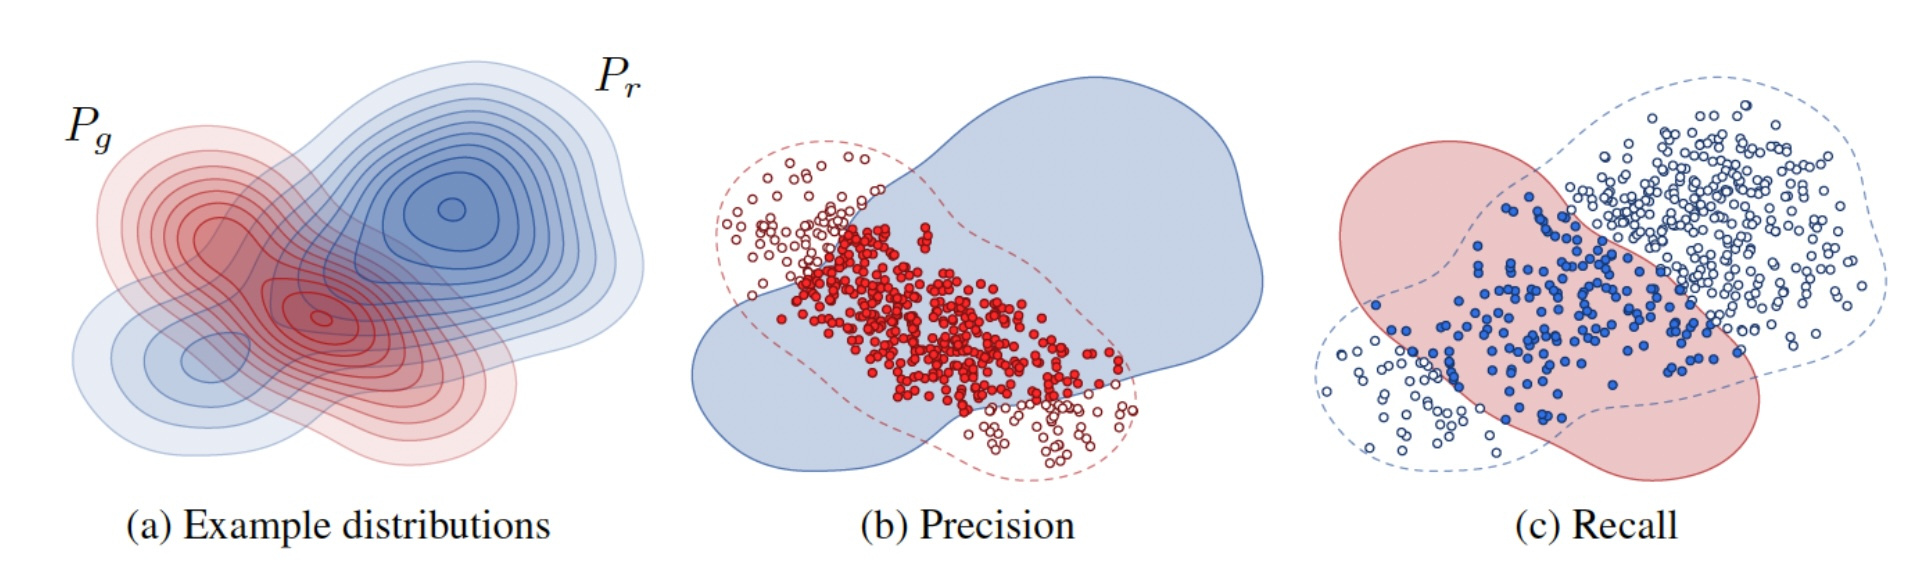
\includegraphics[width=0.7\linewidth]{images/related/precision_recall.jpg}
      \end{center}
      \caption{Precision and Recall. (a) shows the real  distribution $P_r$ and generated distribution $P_g$. (b) Precision: How likely that an image from $P_g$ falls within $P_r$? (c) Recall: How likely that an image from $P_r$ falls within $P_g$? Figure taken from \cite{kynkaanniemi2019improved}}
      \label{fig:precision_recall}
  \end{figure}


However, there are problems associated with these Precision and Recall metrics \citep{naeem2020reliable, alaa2022faithful}.
Notably, they are not robust to outliars in the generative and real datasets. Note that a generative model which only barely 
covers dense modes of the real dataset and overwhelmingly 
produces samples resembling a few real outliars will have perfect precision and recall scores. To adress these, 
\cite{alaa2022faithful} recently proposed $\alpha$-Precision and $\beta$-Recall. $\alpha$-Precision is the 
fraction of generated examples which resemble the "most typical" fraction $\alpha$ of real samples, while  $\beta$-Recall
is the fraction of real samples covered by the most typical fraction $\beta$ of synthetic samples. By varying 
$\alpha$ and $\beta$ from 0 to 1, we can observe the effects of outliars and thus better evaluate the closeness 
of the real and generated distributions. 

\minipar{Authenticity} All of the above metrics are susceptible to a generative model simply "copying and pasting" 
the training data. Also proposed by \cite{alaa2022faithful}, authenticity refers to the rate at which 
a model generates new samples. With  $\alpha$-Precision, $\beta$-Recall and authenticity, \cite{alaa2022faithful}
shows that we can more reliably evaluate generative models compared to existing approaches. 

\minipar{CLIP similarity} In the case of text-guided image editing, the CLIP similarity score uses the 
recent dual CLIP encoder \citep{radford2021learning} which measures the distance in the embedded space 
between the target textual description and the edited image. This score is especially used in recent 
works which perform highly flexible editing \citep{mokady2023null, hertz2022prompt}.

\minipar{LPIPS} 
In the case of image editing, we can measure the LPIPS \citep{zhanglpips2018} score between 
the real image and the edited image. This measures the distance of extracted features between the 
real image and edited image. While editing should change the image slightly, an 
edited image should generally not deviate profoundly from the input image. This metric 
is generally used alongside with other metrics which measure image quality. 

\minipar{Human Evaluation} 
Human evaluation remains a main way of evaluating image quality.  \cite{hype} 
established a standard human benchmark for image evaluation, while other works propose 
more task-specific surveys. \ac{MTurk} remains a popular tool for image editing 
evaluation which allows a diverse pool of humans to choose their preferable 
image edit. 


\subsection{Datasets}

As image editing was historically limited to \ac{GAN}s, datasets used 
for evaluation typically used restricted datasets which could be covered by 
a \ac{GAN}'s domain. Typically, this meant either a validation set of the training 
set, or a different dataset altogether which is similar to the training set.

The most common of these restricted datasets are face datasets, since faces are 
of particular practical use for the public and they present regular structures which 
react better to generation and editing. Common face datasets
include

\begin{itemize}
      \item \textbf{CelebA} \citep{celeba}. It contains 200000 images of celebrity faces of medium-resolution (mostly $178\times218$). Each image is labelled with 40 different binary attributes (e.g. glasses, smile, etc.)
      \item \textbf{CelebAHQ} \citep{karras2018progressive}. A high-resolution extension of the previous dataset, containing 30000 images of $1024\times1024$ resolution.
      \item \textbf{FFHQ} \citep{karra2019stylegan}. Contains 70000 images of $1024\times1024$ resolution scraped from Flikr. This dataset was created to include a much larger variety of faces compared to the previous datasets (which only included celebrities), and includes a variety of ethnicities, genders, ages, and expressions.
\end{itemize} 

Other popular choices for evaluation  include:

\begin{itemize}
      \item Individual subdatasets from \textbf{LSUN} \citep{lsun}. LSUN bedrooms, LSUN Churches, LSUN cars, LSUN horses are popular choices. Each subset dataset contains about 1M images of varying resolution. 
      \item \textbf{Places2} \citep{zhou2017places}, especially a popular choice for training and evaluating inpainting tasks. It contains 10 million labeled images, covering a wide variety of indoor and outdoor scenes. The images are generally of high-resolution.
      \item \textbf{ImageNet} \citep{russakovsky2015imagenet_ilsvrc} about 1.2M images divided into 1000 classes. This dataset can be used for class-based editing.
      \item \textbf{COCO} dataset \citep{caesar2018cocoostuff} for text-based editing. This contains 330000 images, each annotated with 5 captions. 
\end{itemize}

It is worth noting that the recent open-source large-scale diffusion model Stable-Diffusion was trained 
on the public dataset \textbf{LAION-5B} \citep{schuhmann2022laion}. This dataset contains 
5 billion image-text pairs scraped off the web. Text-guided editing methods which use Stable-Diffusion, 
in addition to evaluating on the above datasets, often evaluate on custom-made datasets \citep{bar2022text2live, mokady2023null} of more diverse nature which contain a variety of object categories and 
text prompts for editing.


\section{Our contributions and positioning}

We abord the task of image editing with three different approaches, constituating our three 
contributions. We will present these contributions in the three following chapters, which 
are summarized below.

\paragraph{Chapter 3: Real-Image Editing with a pre-trained \ac{GAN}}

Firstly, we wanted to leverage the existing works on latent-space manipulation for a pre-trained \ac{GAN} 
(\ref{subsection:latent_space_manipulation}). We remarked that existing works performed powerful and 
convincing edits for generated images, but generalized poorly to real images. In order to apply the 
aformentioned techniques to real images, we must first invert the real image into the pre-trained \ac{GAN}
to obtain its corresponding latent code (since \ac{GAN} have no inherent encoder network). Motivated by 
the success of works on latent-space manipulation, we show that we can use a similar technique to 
perform the inversion of a real image, and thus obtain an editable latent code. We extensively 
quantitatively and qualitativly evaluate our method on faces and cars datasets.

\paragraph{Chapter 4: Flexible text-guided image editing}

Although our first contribution works well for images within a pre-trained \ac{GAN}'s  domain, 
editing a more complicated image works poorly. For our second work, FlexIt, we thus took advantage of the 
recently proposed  VQGAN \citep{esser2021taming} (a type of \ac{VAE}) to directly encode images into a codebook of vector-quantized
feature vectors. We optimize this latent space to match the user's target text using the recently proposed 
CLIP dual-encoder \citep{radford2021learning}. Because the \ac{VAE} was not trained to generate images,
its latent code does not capture semantic information like a \ac{GAN} does, and we thus introduce
 a way to efficiently tune our hyper-parameters 
 which encompasses our two 
objectives - (1) obtaining an edited image which matches the target text and (2) minimally changing 
the input image. We thorougly evaluate our method on the ImageNet dataset, showing that with cleverly
tuning of the hyper-parameters, we achieve better results than previous text-guided editing methods.


\paragraph{Chapter 5: Gradient-guided inpainting with a \ac{DDPM}}

We again examined the short-comings of our previous works. While FlexIt can indeed edit any image, 
the \ac{VAE}'s encoder inherently loses original details present in the source image. Moreover,
the lack of generative knowledge within the model can sometimes lead to absurd edits which 
we cannot control. For real-life 
use-cases, this is not permissible. An editing task can be seen as a conditional inpainting 
task, in which the condition only holds effect in the region defined by the inpainting mask. We thus 
aborded the question of inpainting with \ac{DDPM}s. Because of their gradual inference nature, we can 
guarantee zero image fidelity loss in the regions outside of the inpainting mask while continually 
blending the generated output with the known regions through noising and denoising. However, the 
denoising process is too fast for the blending to be successfully harmonized, inspiring works which 
forecfully slow-down the denoising process for better harmonization \citep{lugmayr2022repaint}. We 
go through a different route, and instead guide the denoising process with a gradient of a loss 
specific for harmonization between the two regions. Our method can be applied to unconditional \ac{DDPM}s 
as well as conditional ones, and we performed thorough evaluation on face datasets (CelebaHQ and FFHQ),
 ImageNet, COCO, 
and Places2. 



















% In this chapter, we detail the related work needed to read this thesis. We first briefly
% explain the learning procedure in \acf{DL} and how the data are structured. Then, we describe the main
% \ac{DL} applications and architectures in \acf{CV}. Finally, we introduce the main topic of this thesis
% ---Continual Learning--- and showcase the challenges, benchmarks, and methods of this domain. The
% notations introduced in this chapter and through the thesis are listed in the
% \hyperref[chap:notations]{Notations} section.

% \section{Neural Network Learning}

% Neural Networks are based on the statistical learning theory \citep{vapnik1999statstheory}. In the
% \textit{supervised setting}, the goal of a neural network is to learn the best mapping function $f :
%       \mathcal{X} \rightarrow \mathcal{Y}$ between an input space $\mathcal{X}$ and an output space
% $\mathcal{Y}$.  We consider a \textit{loss} function $\mcL : \mathcal{Y} \times \mathcal{Y}
%       \rightarrow \mathbb{R}^+$ that measures the disagreement between a ground-truth label $y$ and the
% network's prediction $\hat{\vy} = f(\vx)$. In the context of image classification, $\vx$ is the
% image pixels, $y$ is the \textit{class} label of the object present in the image, and $\hat{\vy}$ is
% a vector of probabilities, with one probability per class the model has to predict. The class with
% the highest predicted probability/confidence is chosen as the prediction. Given a \textit{training
%       dataset} $\mathbb{D} = \{(\vx_1, y_1), ..., (\vx_N, y_N)\}$, training a neural network consists in
% finding the set of parameters $\theta_*$ which minimizes the loss function:
% %
% \begin{equation}
%       \theta_* = \operatorname{argmin}_{\theta} \left \{ \frac{1}{|\mathbb{D}|}\sum_{(\vx,y)\in \mathbb{D}} \mcL(f_\theta(\vx), y)\right \}\,.
%       \label{eq:intro_optim}
% \end{equation}
% %
% However, the optimal set of parameters $\theta_*$ minimizing the loss on the training set, can fail
% to predict the correct label on the testing set. Therefore, to avoid this \textit{overfitting}
% phenomenon, regularization functions that limit the parameters space are used as additional
% constraints in addition to the classification loss $\mcL$.

% In practice, the function $f_\theta$ learned by a neural network is composed of a succession of
% linear transformations and non-linear \textit{activation} functions. For example, a simple neural
% network, called \ac{MLP}, here with two layers, could be defined as:
% %
% \begin{equation}
%       \hat{\vy} = f_\theta(\vx) = \operatorname{softmax}(\vW_o \sigma(\vW_h \vx + \vb_h) + \vb_o))\,,
%       \label{eq:intro_mlp}
% \end{equation}
% %
% \noindent with $\vW_h \in \mathbb{R}^{H \times D}$, $\vb_h \in \mathbb{R}^{H}$, $\vW_o \in
%       \mathbb{R}^{C \times H}$, $\vb_o \in \mathbb{R}^{C}$ being the parameters $\theta$ of the
% network. $\sigma$ is a hidden non-linear activation, often a \ac{ReLU}
% ($\operatorname{ReLU(x)} = \text{max}(0, x)$), and $\hat{y} = \operatorname{softmax}(\tilde{\vy}) =
%       \nicefrac{e^{\tilde{\vy}}}{\sum_{i} e^{\tilde{\vy}_i}}$ is the final non-linear activation.

% Likewise, in practice for image classification, the loss is often the categorical cross-entropy:
% %
% \begin{equation}
%       \mcL(\hat{\vy}, \vy) = -\sum_c y_c \log \hat{y}_c\,,
%       \label{eq:intro_ce}
% \end{equation}
% %
% \noindent with $\vy$ a one-hot vector of the labels. Finally, to optimize the parameters of the neural
% network (such as \autoref{eq:intro_optim}), we often use the mini-batch \ac{SGD} algorithm or a variation thereof:

% \begin{algorithm}
%       \begin{algorithmic}[1]
%             \Statex \textbf{input:} a dataset $\mathbb{D}$ with pairs of $(\vx_i, \vy_i)$
%             \Statex \textbf{input:} a loss function $\mcL$
%             \Statex \textbf{input:} a model function $f_\theta$ with $\theta$ the learned parameters
%             \Statex \textbf{input:} a learning rate $\eta$ and a batch size $b$
%             \Statex

%             \While{stopping criterion not satisfied}
%             \State $(\vx, \vy)$ $\gets$ sample mini-batch of size $b$ from $\mathbb{D}$
%             \State Forward pass: $\hat{\vy}$ $\gets$ $f_\theta(\vx)$
%             \State Compute loss: $\mcL$ $\gets$ $\mcL(\hat{\vy}, \vy)$
%             \State Compute the gradients: $\delta$ $\gets$ $\nabla_\theta \mcL$
%             \State Update all parameters: $\theta$ $\gets$ $\theta - \eta \delta$
%             \EndWhile
%       \end{algorithmic}
%       \caption{Procedure to optimize a neural network with gradient descent.}
%       \label{algo:intro_sgd}
% \end{algorithm}

% The learning rate $\eta$ controls the step size when updating the parameters in the direction of the
% gradient. The batch size $b$ defines the number of images seen during one update. The
% \textit{backpropagation} algorithm \citep{rumelhart1986backprop} computes the gradients and the
% update of the parameters. In the case of image classification and segmentation, the main topics
% explored in this thesis, we discern the \textit{feature extractor} from the \textit{classifier} in
% the neural network. The former transforms the input space so that the latter linearly discriminates
% classes. From now on, the feature extractor will be denoted by $f$, and the classifier by $g$ (see
% the \hyperref[chap:notations]{notations}). The model is then $g \circ f$.

% The neural network in \autoref{eq:intro_mlp} can be defined as \textit{shallow} with only one hidden
% layer. By extension, an important success of later neural networks came with training \textit{deep}
% neural network with multiple hidden layers. More generally in this thesis, we will refer to them as
% \acf{DL} models. The majority of \ac{DL} models, in \acf{CV}, in \acf{NLP}, or even in Audio are
% based on the same structure (linear transformations and non-linear activations) and are trained with
% a form of gradient descent.

% \section{Deep Architectures for Computer Vision}
% \label{sec:related_cv}

% A common type of architectures for computer vision is the \acf{ConvNet}. First defined by
% \citet{fukushima1980neocognitron} and then trained with backpropagation by \citet{lecun1999lenet},
% it is a neural network architecture whose linear operators are \textit{convolutions}. While
% handcrafted convolutions \citep{lowe1999sift} rely on well-defined features, a \ac{ConvNet} learns
% the convolution kernels to detect more complex patterns required to minimize the classification
% loss. In 2012, thanks to a large dataset and more efficient code working on \acp{GPU} allowing
% training larger networks, \citet{krizhevsky2012alexnet} won the ILSVC competition
% \citep{russakovsky2015imagenet_ilsvrc} where they had to classify a large dataset ---ImageNet---
% made of 1.28M training images and 1000 classes. From that point forward, multiple improvements were
% made to \acp{ConvNet} \citep{ioffe2015batchnorm,he2016resnet} and these methods have been applied
% not only to classification but also object detection \citep{ren20fasterrcnn}, semantic segmentation
% \citep{chen2018deeplab}, visual question answering \citep{antol2015vqa,benyounes2017mutan}, image
% generation \citep{goodfellow2014gan}, image editing \citep{grechka2021magecally,couairon2022flexit},
% \etc.

% Most \acp{ConvNet} follow a similar structure with blocks of convolutions and pooling. Often, the
% final spatial features are flattened by \ac{GAP} and fed to a linear classifier
% predicting the classes probabilities. \autoref{fig:related_cnn} illustrates this general architecture.

% \begin{figure}[tb]
%       \begin{center}
%             \includegraphics[width=0.8\linewidth]{images/related/cnn.pdf}
%       \end{center}
%       \caption{\textbf{A Convolutional Neural Networks} extracts more complex patterns through its
%             succession of convolutions. \textcolor{Goldenrod}{\textbf{Yellow}} blocks are
%             convolutions, \textcolor{BurntOrange}{\textbf{orange}} blocks are poolings, and the
%             unique \textcolor{ForestGreen}{\textbf{green}} block is the classifier. Given an image,
%             the \ac{ConvNet} can assign to each possible class a probability, all summing to 1. The
%             detected shapes grow in complexity with the depth of the network, from crude edges and
%             textures, to objects. Detected patterns taken from \citet{olah2017feature}.}
%       \label{fig:related_cnn}
% \end{figure}

% \paragraph{Architectures:}The 2010's decade saw major improvements to \acp{ConvNet}, both in their
% architecture and in their training procedure. \citet{srivastava2015highwaynet} and
% \citet{he2016resnet} propose residual connections between blocks likewise: $\vy = \vx +
%       \sigma(\operatorname{Conv}(\vx))$. By reducing the \textit{vanishing gradient} problem
% \citep{hochreiter2001vanishinggrad}, it allows training deeper networks without accuracy
% degradation. This type of connection is now quasi-ubiquitous in all \ac{DL} based architectures.
% Other architecture changes include using convolutions of different kernel sizes in parallel as in
% Inception \citep{szegedy2015inception}, enabling a multi-scales view of the features. These
% architectures are depicted in \autoref{fig:related_resnet_inception}.

% \begin{figure}[tb]
%       \begin{center}
%             \includegraphics[width=\linewidth]{images/related/resnet_inception.pdf}
%       \end{center}
%       \caption{\textbf{Different ConvNet architectures:} \textbf{(a)} illustrates a ResNet-like
%             architecture where there are residual connections between blocks. Used by the vast
%             majority of modern architectures, these connections reduce the vanishing gradient problem
%             and thus enabling the training of deeper networks. \textbf{(b)} showcases an Inception-like
%             architecture where at the same level convolutions with different kernel sizes are used.
%             Each detects patterns of different scales.}
%       \label{fig:related_resnet_inception}
% \end{figure}

% \paragraph{Regularizations:} While the architecture design has an impact on the model performance,
% the training procedure has been shown to be essential in order to reach state-of-the-art results
% \citep{wightman2019resnetstrikesback}. Modern procedures include improvement of \ac{SGD} with an
% adaptive learning rate per layer such as Adam \citep{kingma2014adam}, an improved learning rate
% scheduling, stronger data augmentations
% \citep{muller2021trivialaugment,hingyi2018mixup,zhong2017erasing}, and regularizations such as
% Dropout \citep{gal2016dropout} and stochastic depth \citep{gao2016stochasticdepth}.

% \paragraph{Transformers:} While convolution-based neural networks dominated \acf{CV} in the 2010's
% decade, in the last few years, the transformer architecture gained interest: it was originally
% designed for machine translation in \ac{NLP} \citep{vaswani2017transformer} with an encoder/decoder
% structure and a \textit{self-attention} block between the words embeddings of a sentence. Each word is
% embedded into a high-dimensional vector named a ``\textit{token}''. The self-attention operation of a
% transformer has a quadratic complexity \wrt the number of tokens: in \ac{NLP}, it is manageable
% given a small sentence. However, when applying a transformer on images and considering each pixel
% as a token, the complexity is too important. \citet{dosovitskiy2020vit}, based on the encoder
% structure of BERT \citep{devlin2018bert}, propose instead to consider a patch of pixels as a token,
% reducing significantly the number of tokens.

% \begin{figure}[tb]
%       \begin{center}
%             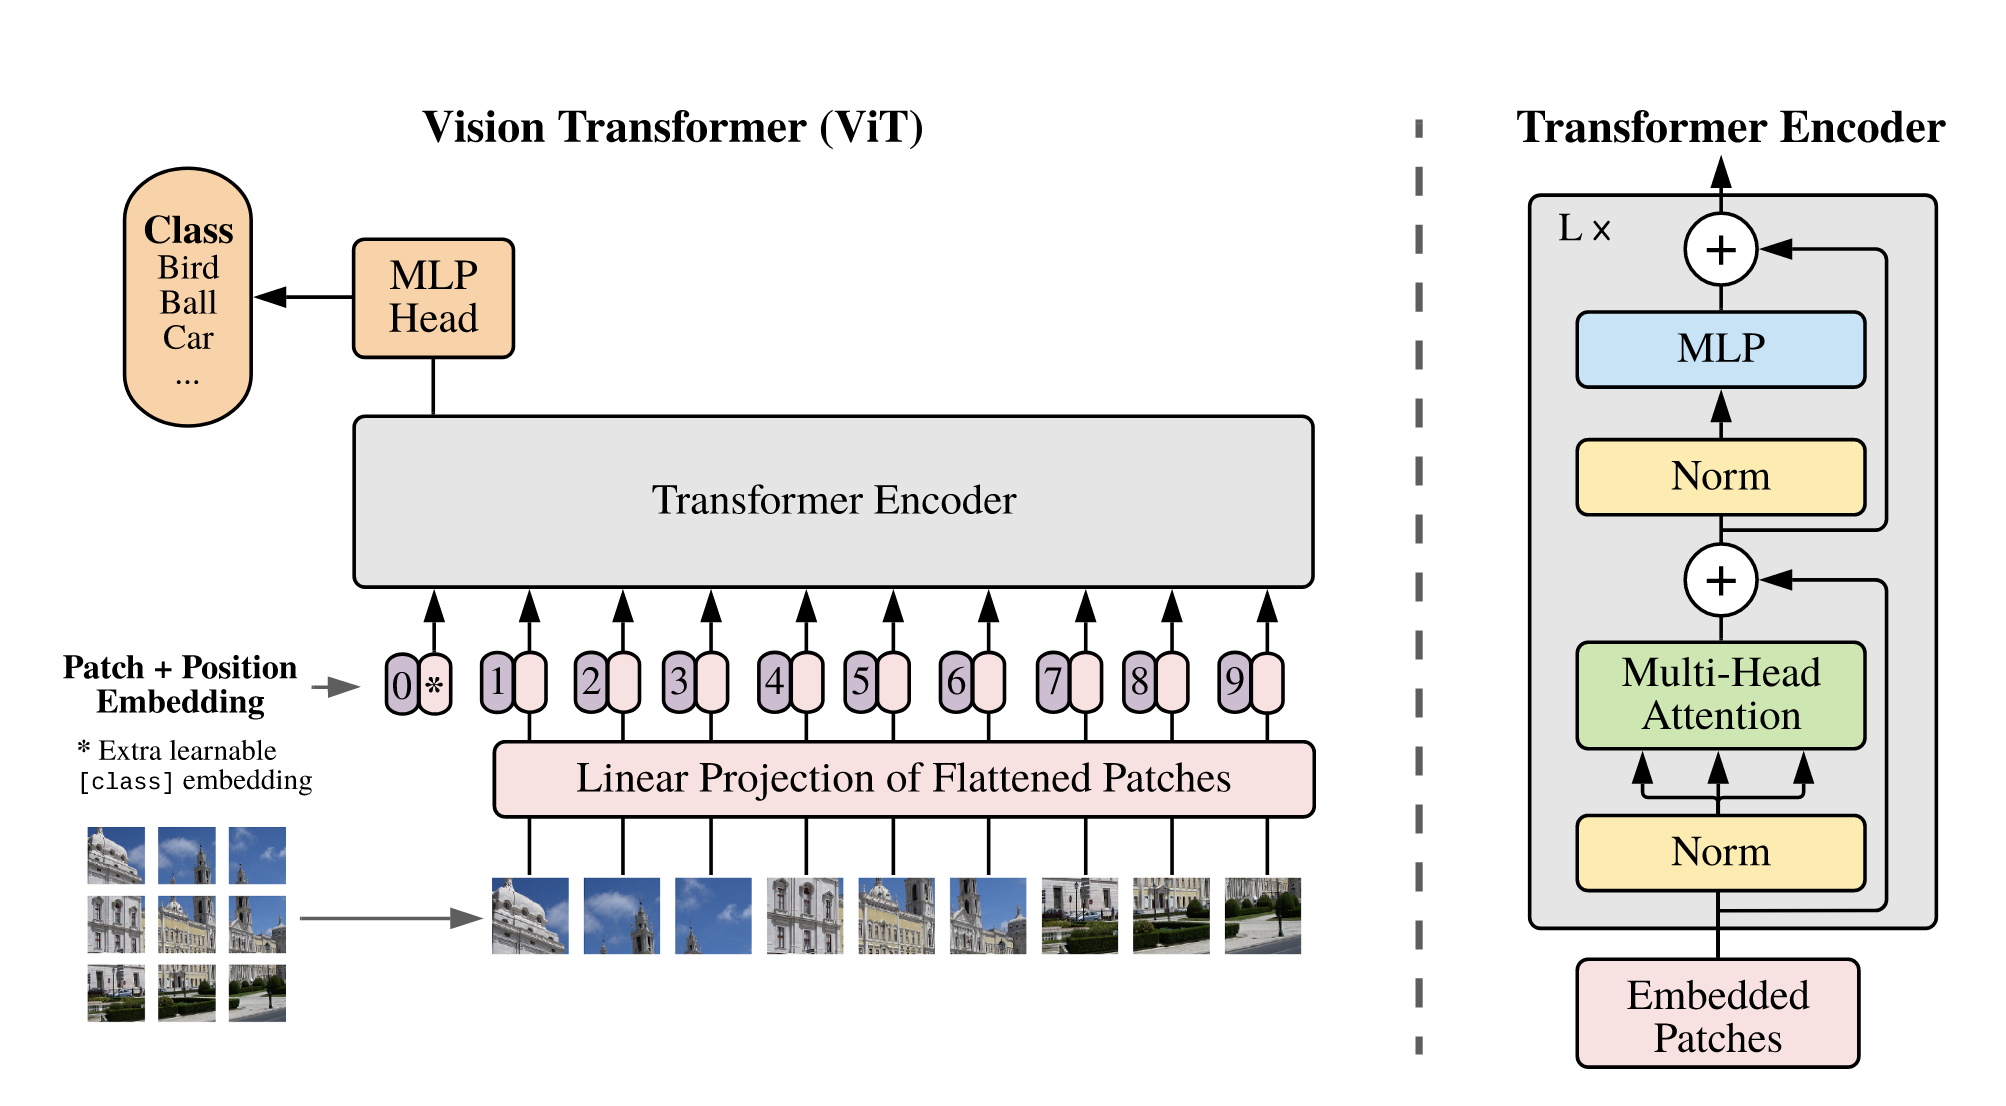
\includegraphics[width=\linewidth]{images/related/vit.png}
%       \end{center}
%       \caption{\textbf{The Vision Transformer (ViT):} the image is cropped without overlap and
%             projected using a convolution whose stride equals the kernel size. A learned ``class
%             token`` is concatenated to the resulting patches, which are then summed with a position
%             embedding. The encoder is made of multiple transformer blocks. Each block is made of two
%             (Layer) Norm layers, a MLP with a single hidden layer, and the Multi-Head Attention
%             block. Finally, only the special ``class token'' is used at the end, and fed to a
%             classifier (here denoted as the ``MLP Head''). Image from \citet{dosovitskiy2020vit}.}
%       \label{fig:related_vit}
% \end{figure}

% This architecture is illustrated in \autoref{fig:related_vit}: we concatenate a special learned
% token, called ``\textit{class token}'', to the patch tokens. Moreover, we also sum these tokens with
% a position embedding to facilitate learning tokens position. Then, successive
% transformer blocks process all the tokens. Each block is made of LayerNorms \citep{ba2016layernorm},
% a self-attention block, a \ac{MLP}, and residual connections. Thus, the self-attention block is:
% %
% \begin{equation}
%       \begin{aligned}
%             Q & =W_{q} \vx\,,                                                       \\
%             K & =W_{k} \vx\,,                                                       \\
%             V & =W_{v} \vx\,,                                                       \\
%             A & =\operatorname{Softmax}\left(Q \cdot K^{T} / \sqrt{D / h}\right)\,, \\
%             O & = W_{o} A V+b_{o}\,,
%       \end{aligned}
%       \label{eq:related_sa}
% \end{equation}
% %
% \noindent $\vx$ are the $N$ patch tokens and the class token, of shape $(N, D)$, $D$ being the
% embedding dimension. The patch tokens are linearly transformed three times in parallel into a
% \textbf{Q}uery, \textbf{K}ey, and \textbf{V}alue. An attention matrix $A$ of shape $(N, N)$ is
% computed from the query $Q$ and the key $K$. Its $i^{\text{th}}$ row contains the similarity between
% the $i^{\text{th}}$ token with all other tokens. Finally, the multiplication between the attention
% matrix and the value matrix $V$ averages all tokens according to their similarities. To extend the
% self-attention to its multi-heads variation (\ac{MHSA}), we use several Query/Key/Value
% transformations, each used in a self-attention on a fraction of the embedding dimension.

% ViT \citep{dosovitskiy2020vit} is the seminal paper on vision transformer. However, its training was
% difficult and needed a large --- and private --- dataset called JFT300M. Later works, including DeiT
% \citep{touvron2021deit} proposed an efficient optimization procedure enabling the training of
% transformers on smaller datasets such as ImageNet \citep{russakovsky2015imagenet_ilsvrc}. Finally,
% multiple works improved also the architecture itself, including CaiT \citep{touvron2021cait}, ConViT
% \citep{dascoli2021convit}, and Swin \citep{liu2021swin}. Notably, PerceiverIO
% \citep{jaegle2021perceiverio} proposed a general architecture whose output is adapted to different
% modalities using specific learned tokens, and whose computation is reduced using a small number of
% latent tokens.

% \section{Continual Learning}
% \label{sec:related_continual}

% Usually, when training a \ac{ConvNet}, we assume the dataset is immutable and \textit{i.i.d.}: no new
% images nor new classes will be learned. The knowledge acquired on one dataset \textit{A} can be
% \textit{transferred} to another dataset \textit{B} with different classes using \textbf{transfer learning}
% \citep{razavian2014transferlearning}. Then, the new model may be efficient on
% the classes of dataset \textit{B} but cannot predict anymore the classes of dataset \textit{A}.

% \textbf{Continual Learning} aims to learn a continually changing dataset without forgetting the
% previous knowledge. The distribution of the dataset continually changes: \eg at each time-step $t
%       \in \{1, ..., T \}$, new
% classes or new samples from potentially new domains are added to the training dataset
% \citep{lomonaco2017core50}. We usually assume the test dataset evolves similarly. Multiple
% distribution drifts exist in Continual Learning
% \citep{morenotorresa2012datasetshift,lesort2021driftanalysis}, and they have been called under
% various names in the literature. Given an input sample $x$ and its ground-truth $y$ (a label in
% image classification, or a segmentation map in semantic segmentation), the major drifts are:

% \begin{itemize}
%       \item \textbf{Covariate drift}: when $p(x)$ changes, it happens with the introduction of new
%             domains \citep{volpi2021continualdomainadapt}.
%       \item \textbf{Prior drift}: when $p(y)$ changes; \ac{CIL} happens with this kind of drift.
%       \item \textbf{Conceptual drift}: when $p(y | x)$ changes. Seldom covered in the literature, it
%             can be found in \acf{CSS}.
% \end{itemize}

% Learning an ever-growing dataset is possible by training from scratch a new model on the union of
% past and new data. However, for multiple reasons like privacy concerns, limited time, or small
% storage capacity \citep{vasquez2017incrementalneuralforest}, there is a restriction on the amount of
% previous data that can be kept. In the extreme case, a model only has access to new data but not old
% data. Evidently, if the initialization of the parameters is random, the model cannot predict
% the past data distribution. However, the new model parameters can be initialized using the
% previous parameters ($\theta^{t} := \theta_*^{t-1}$). Remark, from \autoref{eq:intro_optim}, that
% the optimization procedure of the old ($t-1$) and new ($t$) model is different. Given the average
% loss $L(f_\theta, \mathbb{D}) = \nicefrac{1}{|\mathbb{D}|}\sum_{(\vx,y)\in \mathbb{D}}
%       \mcL(f_{\theta}(\vx), y)$:
% %
% \begin{equation}
%       \begin{aligned}
%             \theta_*^{t-1} & = \operatorname{argmin}_{\theta^{t-1}} \left\{ L(f_{\theta^{t-1}}, \mathbb{D}^{t-1})\right \}\,, \\
%             \theta_*^{t}   & = \operatorname{argmin}_{\theta^{t}} \left\{ L(f_{\theta^{t}}, \mathbb{D}^{t})\right \}\,,       \\
%       \end{aligned}
%       \label{eq:intro_forgetting_weights}
% \end{equation}
% %
% where the loss is minimized respectively with respect to the old ($\mathbb{D}^{t-1}$) and new
% dataset ($\mathbb{D}^{t}$). Evidently, the optimal parameters $\theta_*$ are different for the task
% $t$ and $t-1$. This difference results in what we call a \textit{forgetting}: $\theta_*^t$ is
% optimal for the new task $t$ but is suboptimal for the task $t-1$, therefore performance on the
% previous task may be degraded ($L(f_{\theta^{t}}, \mathbb{D}^{t-1}) \gg L(f_{\theta^{t-1}},
%       \mathbb{D}^{t-1})$). This performance drop is actually so important that the literature names it a
% \textbf{Catastrophic Forgetting} \citep{robins1995catastrophicforgetting}. It is particularly
% critical in the context of image classification where each new task brings new classes to be
% classified as described below.

% \begin{figure}[tb]
%       \begin{center}
%             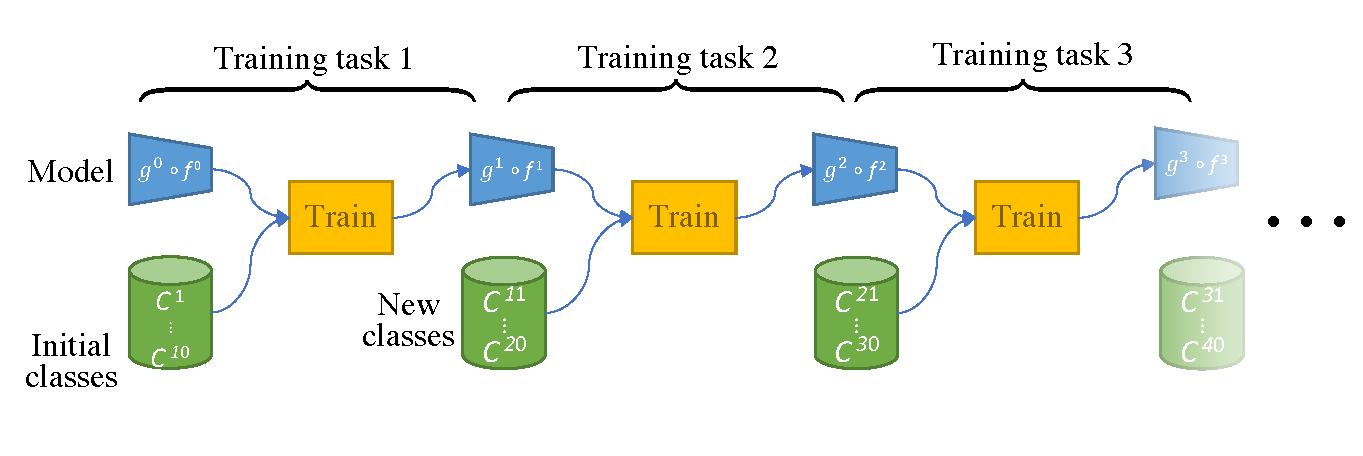
\includegraphics[width=1.0\linewidth]{images/related/protocol}
%       \end{center}
%       \caption{\textbf{Training protocol for incremental learning}. At each training task we learn a
%             new set of classes, and the model must retain knowledge about \textit{all} classes. The
%             model is allowed a \textit{limited} memory of samples of old classes.}
%       \label{fig:related_protocol}
% \end{figure}

% \paragraph{Class-Incremental Example} More concretely, a common benchmark in \acf{CIL} is learning
% the image classification CIFAR100 dataset \citep{krizhevskycifar100}, made of 100 classes, in
% multiple steps, each made of several new classes. During the first step $t=1$, the model $g^1 \circ
%       f^1$ learns the first 10 classes $\mcC^{t=1}$. During the second step $t=2$, the model $g^2 \circ
%       f^2$ is initialized from the learned parameters of the previous model $g^1 \circ f^1$ and learns the
% next 10 classes $\mcC^{t=2}$., and so on, until all 100 classes are learned at the last step $t=T$.
% After each step, we evaluate the model on the testing data of all seen classes $\mcC^{1:t}$.
% \autoref{fig:related_protocol} illustrates such continual protocol, and
% \autoref{fig:related_forgetting} depicts the continual performance of a both trained from scratch on
% all data for each task and a continual model finetuned only on new data. The continual model
% over-predicts new classes \citep{davidson2020masteryincremental} and has a low overall accuracy due
% to a forgetting of old classes. This clearly illustrates how important is the catastrophic
% forgetting. While in this thesis we mainly tackle \acf{CIL} benchmarks, we describe other continual
% benchmarks in detail in the appendix (\autoref{sec:related_variation}).

% \begin{figure}[tb]
%       \begin{center}
%             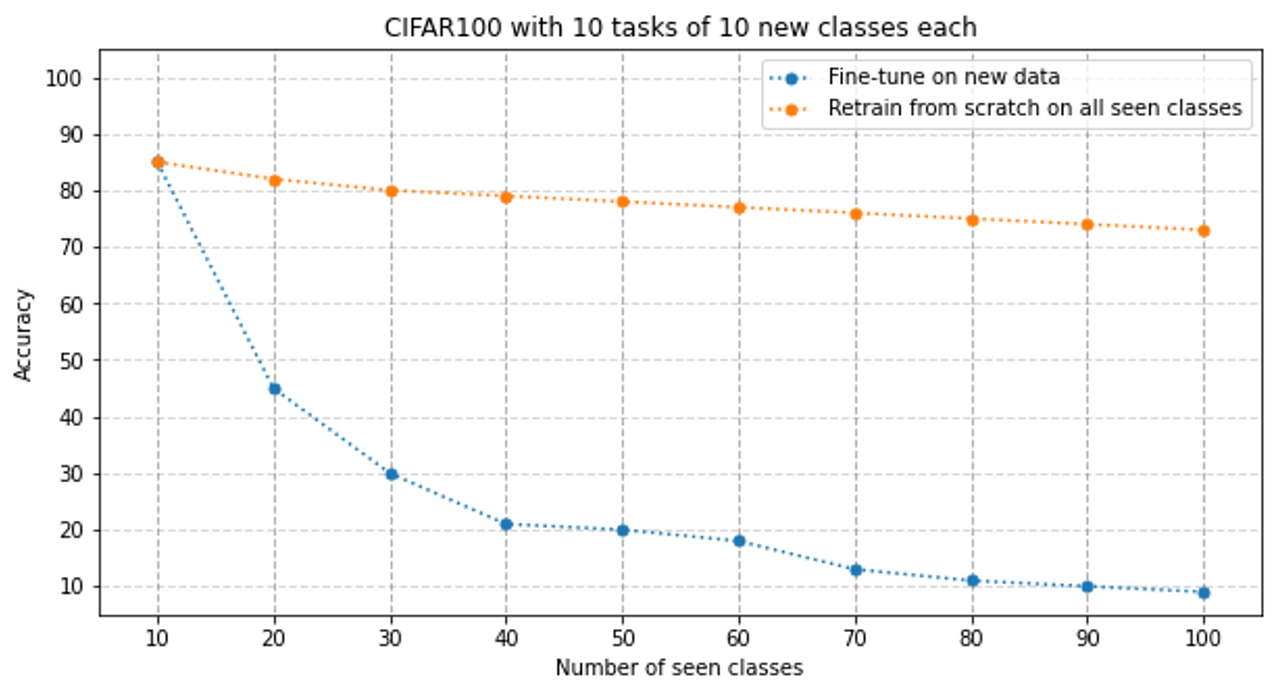
\includegraphics[width=0.8\linewidth]{images/related/catastrophic_forgetting.png}
%       \end{center}
%       \caption{\textbf{Illustration of the forgetting in Class-Incremental Learning}.
%             \textcolor{orange}{orange} line displays the accuracy of a model which is re-trained from
%             scratch at each step on all previous training data $\mcC^{1:t}$. This model, usually called
%             Joint, is considered as a reasonable upper bound. On the other hand, the
%             \textcolor{blue}{blue} line is a model finetuned solely on new classes $\mcC^{t}$ without
%             access to previous classes $\mcC^{1:t-1}$. The gap between both models illustrates the
%             catastrophic forgetting.}
%       \label{fig:related_forgetting}
% \end{figure}

% \paragraph{Single-Head \vs Multi-Heads} are the two main evaluation settings in Continual Learning
% \citep{chaudhry2018riemannien_walk}. In the former setting, a model has to classify samples among
% all seen classes $\mcC^{1:t}$, that could have been learned from any of the seen steps. On the other
% hand, in a multi-heads setting, a model knows at test-time the step/task identifier $i$ of the
% samples. Thus, it only has to classify among the limited number of classes brought by a step
% ($\mcC^i$). Multi-Heads evaluation is closely related to multi-tasks learning. During this thesis,
% we focus on the Single-Head evaluation because it is more realistic as it is rarely possible to know
% from which step a sample comes from in a real-life setting. This setting is also more challenging
% because a unique classifier must discriminate among all tasks' classes instead of having a different
% classifier per task \citep{lesort2019regulshortcomings}.


% %\subsection{Metrics for Continual Learning}
% \label{sec:related_metrics}

% \paragraph{Metrics} Multiple metrics exist in Continual Learning: the most common are the
% \textbf{final accuracy} and \textbf{average incremental accuracy}. The former measures the
% performance of the model on all tasks at the last step, the latter measures the average of
% performance on all seen tasks after each new task learned \citep{rebuffi2017icarl}. Practically,
% given $A_{i,t}$ the accuracy of the $i^{th}$ task after learning the $t^{th}$ task, the final
% accuracy is (assuming balanced tasks):
% %
% \begin{equation}
%       \text{Acc}_F = \frac{1}{T} \sum_{i=1}^T A_{i,T}\,,
%       \label{eq:related_final_acc}
% \end{equation}
% %
% and the average incremental accuracy:
% %
% \begin{equation}
%       \text{Acc}_a = \frac{1}{T} \sum_{t=1}^T \frac{1}{t}  \sum_{i=1}^t A_{i,t}\,.
%       \label{eq:related_avg_acc}
% \end{equation}
% %
% Average incremental accuracy is somewhat more important than simply the final accuracy: a continual
% model should be good after every step because in a true continual setting, there is not a ``final
% task''.

% Other metrics exist \citep{diaz2018continualmetrics}, such as \textbf{forgetting}
% \citep{chaudhry2018riemannien_walk} which records how much a model has lost performance-wise on a
% task compared to the first time it has learned it. The interest of this metric is to be agnostic of
% the absolute performance of the model used.

% Finally, metrics such as \textbf{speed} (\ie the number of images processed per second) or used
% \textbf{capacity} (\ie number of learned parameters) are important:
% \citet{ramasesh2022scalecontinual} recently showed that the larger a model was the lower was the
% forgetting.

% \section{Methods to reduce forgetting}
% \label{sec:related_methods}

% Multiple approaches exist to reduce forgetting in Continual Learning. The major ones are
% rehearsal of old data (\autoref{sec:related_rehearsal}), regularizations constraining the model's
% behavior (\autoref{sec:related_regul}), and structural adaptations (\autoref{sec:related_structural}).

% \subsection{Rehearsal Learning}
% \label{sec:related_rehearsal}

% The most efficient method to reduce forgetting is \textbf{rehearsal learning} where old samples will
% be seen alongside the new samples. The amount of old samples stored is extremely limited, otherwise,
% it would defeat the purpose of continual learning. \autoref{fig:related_protocol_rehearsal} illustrates how
% rehearsal learning happens in Continual Learning. During the first step, a model is trained on all
% available samples. Then, it stores a limited amount of those in a \textit{memory}. During the second
% step, the model has access to new samples but also all samples stored in the memory. In
% Class-Incremental, an equal amount of samples per class is stored in memory. There are
% two major approaches to determine this amount: \citet{rebuffi2017icarl} propose to fully use a
% memory of size $\mcM$ among all $\mcC$, while \citet{hou2019ucir} instead kept fixed the number of
% samples stored per class to $\nicefrac{\mcM}{|\mcC^{1:T}|}$.

% \begin{figure}[tb]
%       \begin{center}
%             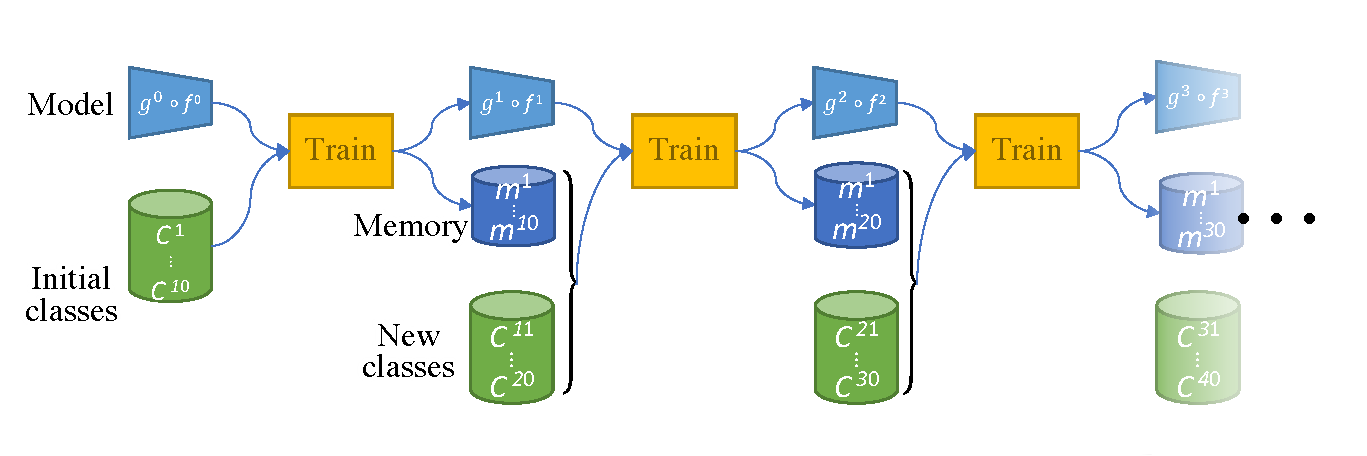
\includegraphics[width=1.0\linewidth]{images/related/rehearsal}
%       \end{center}
%       \caption{\textbf{Training with a rehearsal memory}. After each task a fraction of the
%             data is stored in a memory to be used in the next task. Rehearsal learning is the most
%             efficient method to reduce forgetting, but unfortunately the memory capacity is often
%             extremely limited.}
%       \label{fig:related_protocol_rehearsal}
% \end{figure}

% \paragraph{Herding} is the action of choosing which samples per class to store in the rehearsal
% memory. The most naive herding method is to randomly sample images. Despite its simplicity, it is
% quite competitive with more complex method \citep{castro2018end_to_end_inc_learn}, echoing similar
% results in \ac{AL} \citep{gal2017activelearning}. Other herding methods include fetching samples
% close to the class mean in the feature space \citep{castro2018end_to_end_inc_learn} or close to an
% incremental barycenter \citep{rebuffi2017icarl}.

% \paragraph{Sampling} is an important but yet fewly investigated topic in Continual Learning. Most
% models mix all memory samples with new samples without any under- or over-sampling.
% \citet{castro2018end_to_end_inc_learn} propose to finetune for a few epochs, after training on a new
% step, on a balanced set of old and new classes samples. \citet{chaudhry2019tinyepisodicmemories}
% oversample tiny memory with as low as one sample per class, and show, in the context of Online
% Learning where models learn in only one epoch, that continual models still do not overfit. In the
% same context, \citet{aljundi2019maximallyinterfered} propose to over-sample the memory examples with
% the highest losses. In an imbalanced situation for Continual Learning, over- and under-sampling can be
% applied depending on the number of samples per class \citep{kim2020imbalancedcontinual}.

% \paragraph{Efficient Storing} is important for rehearsal learning: a bigger rehearsal memory leads
% invariably to less forgetting \citep{hou2019ucir}. Thus, multiple works consider how to store more
% rehearsal samples given the same memory size: \citet{hayes2020remind} compress intermediate features
% of memory samples with a lossless compression algorithm.
% \citet{iscen2020incrementalfeatureadaptation} also store features but modify them through the
% training to handle the inherent internal covariate drift.

% \paragraph{Pseudo-rehearsal} does not need to store samples but instead generates pseudo-samples for
% rehearsal \citep{lesort2019generative}. The generation can be done with auto-encoders from
% intermediate features \citep{kemker2018fearnet,ayub2021eec} or use \ac{GAN}
% \citep{shin2017deep_generative_replay}. Unfortunately, those methods have several drawbacks: they
% struggle to scale to large images, the generator size may be superior to a classic rehearsal memory
% size which would defeat the goal of using less storage, and finally, the generator may itself suffer
% from catastrophic forgetting \citep{zhai2019lifelonggan}. \citet{liu2020mnemonics} propose instead a
% method halfway between rehearsal and pseudo-rehearsal: the authors randomly sample real images, and
% then during continual training, slightly modify them via bi-level optimization
% \citep{wang2018datasetdistillation} to minimize forgetting.


% \subsection{Regularization-based Approaches}
% \label{sec:related_regul}


% \begin{figure}[tb]
%       \begin{center}
%             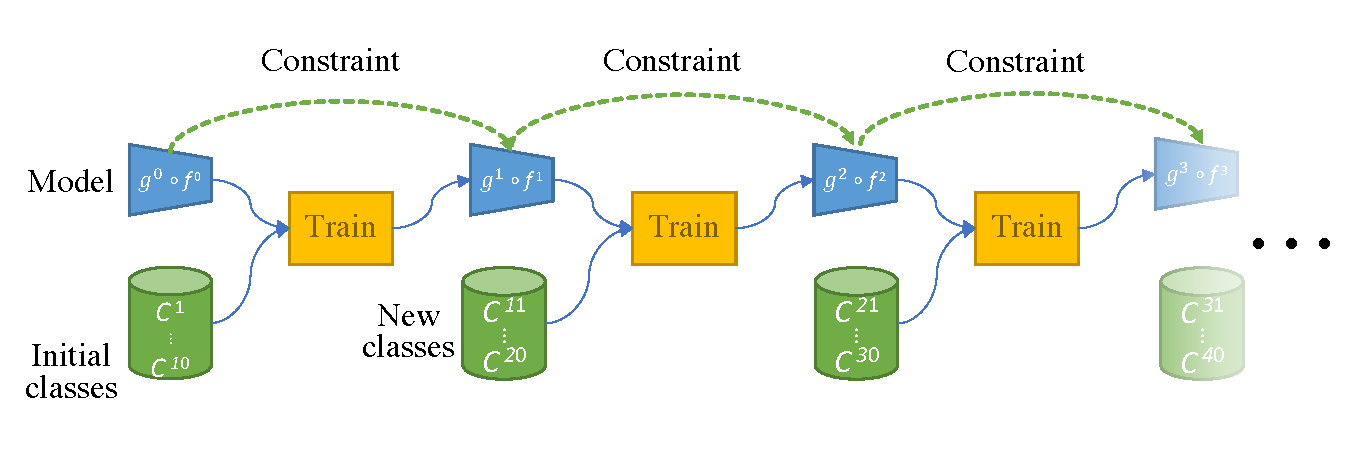
\includegraphics[width=1.0\linewidth]{images/related/constraints}
%       \end{center}
%       \caption{\textbf{Constraining the new model based on the old model}. During each task, after
%             the first one, the new model is constrained to be similar to the old model in order to reduce
%             forgetting.}
%       \label{fig:related_protocol_constraints}
% \end{figure}

% A common and efficient way to reduce forgetting is to minimize the difference in behavior between
% the old and new models as illustrated in \autoref{fig:related_protocol_constraints}. These constraints can be
% expressed through various forms and are described below.

% \subsubsection{Weight-based constraints}
% \label{sec:related_regul_weight}


% The most straightforward way to avoid completely forgetting is that the old and new models stay
% identical. While the model would be \textit{rigid} (no forgetting), it is also not \textit{plastic}
% (changing a lot) at all, and thus cannot learn any new tasks. Thus, a line of research proposed to
% constrain only a portion of the neurons:
% %
% \begin{equation}
%       \mcL(\theta^t, \theta^{t-1}) = \mcL_t(\theta^t) + \lambda \sum_i \Omega_i^{t-1} (\theta^t_i - \theta_i^{t-1})^2\,,
%       \label{eq:related_weight_constraint}
% \end{equation}
% %
% where $\mcL_t(\theta)$ is the loss at the current task $t$ (\eg the cross-entropy), $\theta_i^t$
% and $\theta_i^{t-1}$ respectively the $i^\text{th}$ neuron of the current and previous model, and
% $\Omega_i^{t-1}$ a neuron-wise importance factor. The intuition is that important neuron for the
% previous task $t-1$ should not change, while the others can be adapted to fit the new task $t$.

% \citet{kirkpatrick2017ewc}, followed by \citet{zenke2017synaptic_intelligence} and
% \citet{chaudhry2018riemannien_walk} propose to use the diagonal Fisher information matrix as
% importance factors. The motivation behind was that the posterior $p(\theta^{t-1} | \mcD^{t-1})$ must
% contain the information about which parameters are important to the previous dataset $\mcD^{t-1}$.
% This posterior can be approximated by a Gaussian distribution whose diagonal precision is given by
% diagonal Fisher information matrix. A higher value means a more important neuron for the previous
% task, and thus the constraint should be increased proportionally. Thus, a lower value, for a less
% important neuron, means that it can change drastically, which would facilitate learning new data.
% This strikes a balance between rigidity (not changing and thus not forgetting), and plasticity
% (changing, and thus learning new concepts). Note that \citet{aljundi2018MemoryAwareSynapses} instead
% use the sensitivity of the model when small perturbations are added to the neurons to measure their
% importance.

% However, it is worth remarking that weight-based constraints are usually limited to the multi-heads
% setting where a task identifier is available at test time. \citet{lesort2019regulshortcomings} show
% that in the single-head setting, they struggle to reduce forgetting and are significantly
% outperformed by the simple (but somewhat memory costly) rehearsal learning.

% \subsubsection{Gradient-Based methods}
% \label{sec:related_regul_gradient}

% \begin{figure}[tb]
%       \begin{center}
%             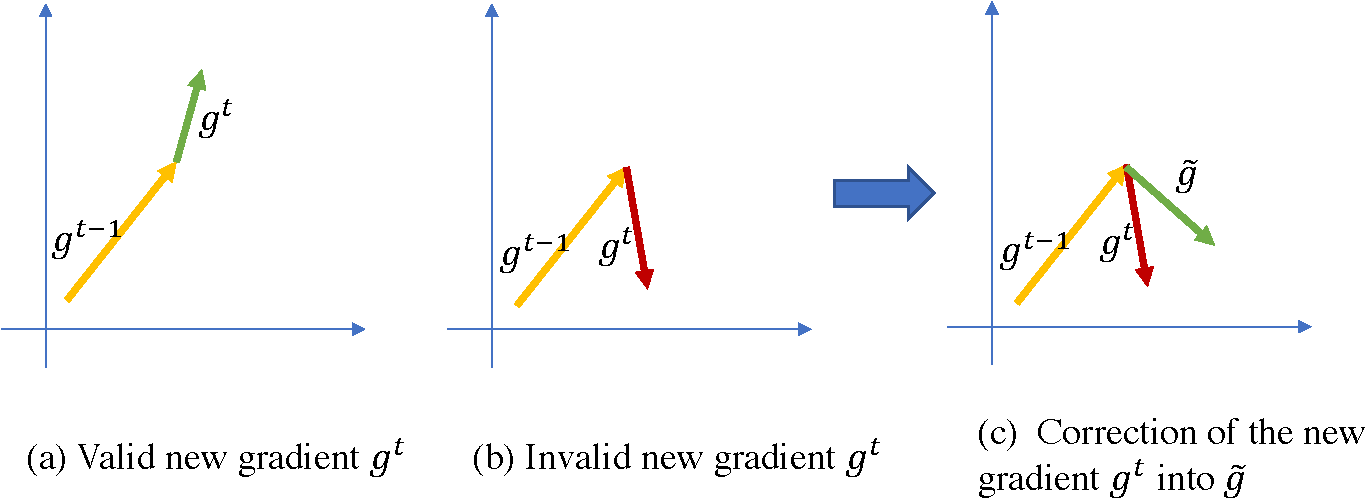
\includegraphics[width=1.0\linewidth]{images/related/gem.pdf}
%       \end{center}
%       \caption{\textbf{GEM's gradient constraint} forcing updates to be in the same direction as the
%             gradient \wrt old samples. In (a) the new gradient $g^t$ is valid, while in (b) the new gradient
%             violates the constraint of $\langle g^t,\, g_{t-1}\rangle \ge 0$. In (c), the invalid gradient
%             $g^t$ is projected to the closest valid alternative $\tilde{g}$.}
%       \label{fig:related_gem}
% \end{figure}

% \citet{lopezpaz2017gem} propose the GEM model that combines a constraint on the gradients and
% rehearsal learning. The algorithm requires that the loss on a given stored sample must not increase
% despite the model learning new classes. The authors, given a locality assumption, rewrite this
% formulation as enforcing that the gradient of a new sample ($g$) to be in the same \textit{direction} as
% the gradient of all stored old samples ($g_i \, \text{for all}\, i \in \mcM$):
% %
% \begin{equation}
%       \langle g,\, g_i\rangle \ge 0,\, \text{for all}\, i \in \mcM\,,
% \end{equation}
% %
% \noindent with $\mcM$ the rehearsal memory. If the constraint is violated, the new gradient $g$ is
% projected to the closest in L2 norm gradient that satisfies the angle constraint by minimizing a
% quadratic program. The constraint is illustrated in \autoref{fig:related_gem}. The drawback of this
% method is the computational cost that can grow prohibitively when the memory is too large.
% \citet{chaudhry2019AGEM} propose Averaged-GEM to speed up GEM: the authors do not constraint the
% gradient of individual memory samples but only the average of all memory samples.
% \citet{aljundi2019gradientselection} also improved GEM's speed by selecting only a subset of the
% memory samples that maximize the feasible region.

% Differently, but still constraining the gradients: \citet{farajtabar2020ogd}'s OGD forces the gradients of
% task $t$ to be orthogonal to gradients of task $t-1$. They use the Gram-Schmidt procedure to
% orthogonalize the new gradients, allowing updates for the new task that minimally interfere with the
% performance of old tasks. \citet{saha2021gpm}'s GPM does likewise but uses instead a k-rank
% approximation of the SVD of the representation matrix.


% \subsubsection{Output-based constraints regularizations}
% \label{sec:related_regul_output}

% Finally, the majority of Continual models that are benchmarked on large datasets (\eg ImageNet
% \citep{deng2009imagenet}) use a combination of rehearsal
% learning (\autoref{sec:related_rehearsal}) and constraints on the model's outputs.

% LwF \citep{li2018lwf} and iCaRL \citep{rebuffi2017icarl} apply the \ac{KD}
% \citep{hinton2015knowledge_distillation} on the model's probabilities. It usually consists in
% minimizing the \ac{KL} between the probabilities of the old and new models:
% %
% \begin{equation}
%       \mcL_\text{KD} = \operatorname{KL}(\operatorname{softmax}(\frac{\tilde{y}^{t-1}}{\tau}) \Vert \operatorname{softmax}(\frac{\tilde{y}^t}{\tau})\,,
% \end{equation}
% %
% where $\tilde{y}^{t-1} = g^{t-1} (f^{t-1}(\vx))$ and $\tilde{y}^{t} = = g^{t} (f^{t}(\vx))$ are respectively the logits of the old and new model,
% and $\tau$ a \textit{temperature} to soften the probabilities in order to give more importance to
% the model confidence in other classes than the top one. These probabilities, nicknamed \textit{dark
%       knowledge} by \citet{hinton2015knowledge_distillation}, contain additional information about the
% model which are useful to distil. Note that in the context of Class-Incremental, the new model
% predicts more classes than the old model, therefore, the \ac{KL} is only applied on the logits
% common to both the old and the new models. The \ac{KD} is sometimes also defined as the binary
% cross-entropy between the sigmoid-activated logits.

% Constraining the probabilities is now so ubiquitous that most models include it in their base
% losses. On the other hand, a few models considered constraining intermediate outputs. MK2D
% \citep{peng2019m2kd} uses the \ac{KD} from both the final classifier and an auxiliary classifier
% similarly to the Inception network \citep{szegedy2015inception}. \citet{hou2019ucir} maximize the
% cosine similarity between the embeddings produced by the \ac{GAP}.
% \citet{dhar2019learning_without_memorizing_gradcam} minimizes the L1 distance between the attention
% maps produced by GradCam \citep{selvaraju2017gradcam}.

% \subsection{Structural Strategies}
% \label{sec:related_structural}

% \begin{figure}[tb]
%       \begin{center}
%             {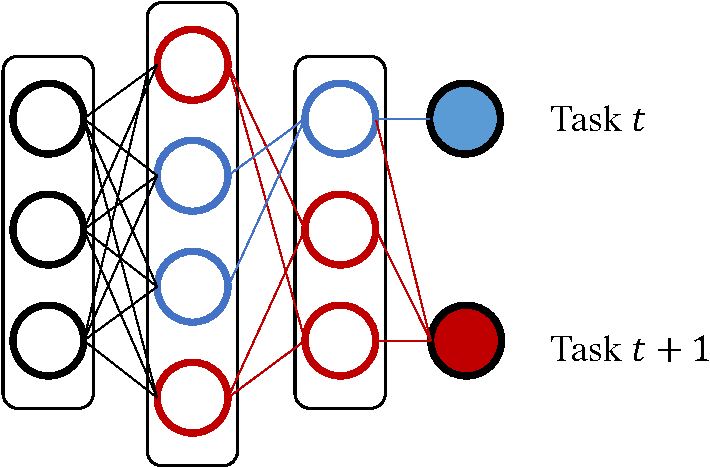
\includegraphics[width=0.5\linewidth]{images/related/subnetworks.pdf}}
%       \end{center}
%       \caption{\textbf{Task-specific subnetworks} that can be uncovered with a sparsity loss or
%             learned masking. \textcolor{blue}{\textbf{Blue}} neurons are dedicated to
%             the task $t$, \textcolor{red}{\textbf{red}} neurons to the following task
%             $t+1$, and \textbf{black} neurons are shared among all tasks. At
%             test-time, a task identifier of the sample is required to select the
%             right subnetwork path.}
%       \label{fig:related_subnetwork}
% \end{figure}

% Multiple works also propose to adopt dynamic strategies where the configuration of the neural
% network evolves after each task. Critically, not only the number of neurons changes in the classifier $g^t$
% (to incorporate new classes to predict), but the feature extractor $f^t$'s neurons count or organization
% will also differ from its previous iteration $f^{t-1}$.


% \paragraph{Subnetworks} The Lottery Ticket Hypothesis \citep{frankle2019lottery_ticket} states that
% subnetworks made of a fraction of the neurons and connections of a larger network, can reach
% excellent performance. Several Continual Learning models exploit that property by using a
% subnetwork per task. Those subnetworks can be uncovered via genetic algorithms
% \citep{fernando2017path_net}, via induced L1 sparsity \citep{golkar2019neural_pruning}, or even
% learned masked \citet{serra2018hat,hung2019cpg}. Usually, these methods require a task identifier at
% test-time in order to select the right subnetwork (see \textit{multi-heads} in
% \autoref{sec:related_continual}). Later, \citet{wortsman2020supermasks} propose to infer the task
% identifier by selecting the subnetwork with the lowest entropy. This subnetwork-based approach is
% illustrated in \autoref{fig:related_subnetwork}.

% \paragraph{Dynamically Expandable Networks} A neural network can also be expanded through its continual
% training to accommodate the growing amount of tasks to solve. First, \citet{rusu2016progressive}
% propose to have one network per task, where the $i^{\text{th}}$ network would depend both on the
% input and all previous networks' intermediate features. Unfortunately, memory consumption is
% quickly prohibitive with many tasks. Following works propose to only add blocks of parameters,
% and only when deemed necessary \citep{veniat2021mntdp}. While these dynamic networks often require
% an identifier at test-time to select the right subset of parameters, recently, DER
% \citep{yan2021der} removed this need by learning a classifier upon the concatenated features of all tasks:
% Their dynamic expansion of the representation adds a new feature extractor per task. All
% extractors' embeddings would then be concatenated and fed to a unified classifier, discarding the
% need for a task identifier at test-time. To limit an explosion in the number of parameters, they
% aggressively prune each model after each task using the HAT \citep{serra2018hat} procedure.
% Unfortunately, the pruning is hyperparameter sensitive. Therefore, hyperparameters are tuned
% differently on each experiment: for example, learning a dataset in 10 steps or in 50 steps use
% different hyperparameters. While being impracticable, it is also unrealistic because the number of
% classes is not known in advance in a true continual situation. Simple-DER \citep{li2021preserve}
% also uses multiple extractors, but its pruning method doesn't need any hyperparameters; the negative
% counterpart is that Simple-DER controls less the parameter growth.

% \paragraph{Task Conditioning} Rather than adding many new parameters, it is also possible to only
% add a few parameters that will adapt the existing network behavior for a task.
% \citet{rebuffi2017visualadapters} propose to add a different residual per task: given a task
% identifier, the associated residual is used, and the features are modulated to best fit the given
% task. Instead of adapting the features, \citet{wen2020batchensemble} and \citet{sun2019metatransfer}
% propose to share most of the weights across tasks, but have task-specific weights that directly
% modify the shared weights.

% \paragraph{Mixture-of-Experts} Mixture of experts \citep{masoudnia2014mixture} have also been
% proposed, where multiple experts combine their decision. \citet{aljundi2017experts} learn a gating
% system to use the right task-specific expert. \citet{collier2020routingnetwork} stress the importance
% on sharing experts when tasks are similar.
% %\citet{yan2021der} and \citet{li2021preserve} proposed
% %to have a \ac{ConvNet} per task and to concatenate their output embeddings to be fed to a single
% %classifier. To avoid parameters explosion, they aggressively prune each \ac{ConvNet}.

% \paragraph{Classifier Correction} Forgetting happens in both the feature extractor and the
% classifier. Previously described rehearsal and regularization methods try to reduce it in both
% places. On the other hand, multiple works focus solely on the classifier. They remark that in
% \acf{CIL}, the classifier is miscalibrated \citep{guo2017miscalibration} where the model
% over-predicts new classes to the detriment of old classes. \citet{belouadah2019il2m} compensate the
% bias towards new classes by rectifying predictions of past classes using their recorded accuracies
% and confidences. \citet{wu2019bias_correction} learn a linear model on validation data to recalibrate
% the logits of the new classes. \citet{zhao2020weightalignement} normalizes the norm of the classifier
% weights associated with new classes so that their average norm becomes the same as that for old
% classes. \citet{hou2019ucir}, aims for a similar result by replacing the dot product in the
% classifier with the cosine similarity, resulting in unit norm classifier weights.

% \section{Positioning}

% Continual Learning encompasses very different benchmarks and methods. In this PhD thesis, we tackle
% multiple types of continual drift using different approaches. All the proposed strategies consider
% the intermediary features of a neural network to reduce catastrophic forgetting. We summarize
% below the three main chapters:

% \paragraph{Feature-based Regularizations} First in \autoref{chapter:regularization}, we consider
% \acf{CIL} scenarios with a prior drift where new classes are continually added. In this setting, our
% approach consists in rehearsal learning (\autoref{sec:related_rehearsal}) and output-based
% regularizations (\autoref{sec:related_regul_output}). Previous works reduced forgetting by
% constraining either the final probabilities of the classifier \citep{li2018lwf} or the ultimate
% embedding of the feature extractor \citep{hou2019ucir,dhar2019learning_without_memorizing_gradcam}.
% In a first section (\autoref{sec:podnet}), we propose instead a regularization applied on several
% intermediary levels of the features extractor. Moreover, few considerations have been made on how
% the regularization loss makes the model more rigid, leading to less forgetting on old classes but
% also impacting negatively the learning of new classes. Instead, we carefully define a regularization
% loss, through pooling, balance effectively the performance of old and new classes. In a second
% section (\autoref{sec:ghost}), we consider if the forgetting could be avoided preemptively.
% \citet{aljundi2019selfless} consider allocating extra capacity implicitly in the learned feature
% space for future classes using an unsupervised sparsity loss. Differently, we choose to draw from
% weak metadata of the future unseen classes \citep{hanrebuffi2020autodiscovering} to estimate their
% representation and thus explicitly allocate capacity, reducing forgetting before it even happens.

% \paragraph{Continual Semantic Segmentation} Second, in \autoref{chapter:segmentation}, we tackle
% \acf{CSS}. In this benchmark, defined recently by \citet{cermelli2020modelingthebackground}, images
% have a label per pixel, and only the current classes are labelized. Thus, both the prior and concept
% drifts happen where new classes are added but also the signification of a pixel can change through
% time. In this setting, all previous works only considered regularizations
% (\autoref{sec:related_regul_output}) based on the final probabilities
% \citep{michieli2019ilt,cermelli2020modelingthebackground}. Instead, we expand from our previous
% chapter to consider the multi-scale intermediary features. Moreover, no work directly tackled the
% partial labelization of the images \citep{cermelli2020modelingthebackground}. We propose for this
% challenge an uncertainty-based pseudo-labeling \citep{saporta2020esl}, and a new rehearsal method
% (\autoref{sec:related_rehearsal}), optimized for segmentation.

% \paragraph{Dynamic Transformers} In this third and last chapter (\autoref{chapter:dynamic}), we only
% aim to solve the prior drift but using a method radically different from previous chapters: dynamic
% networks (\autoref{sec:related_structural}). Previous dynamic networks usually expand their capacity
% by a large margin during the continual training to handle the growing amount of tasks to learn
% \citep{yan2021der}. To avoid a parameter count unbounded growth, the models are usually pruned
% aggressively. The main drawback of these methods is that the pruning can still result in models too
% large and often need careful finetuning of hyperparameters. We propose in this chapter, a dynamic
% expansion based on the transformer architecture with almost no memory overhead contrary to
% concurrent works, that conditions \citep{perez2018film} the intermediary features.
